%%%%%%%%%%%%%%%%%%%%%%%%%%%%%%%%%%%%%%%%%%%%%%%%%%%%%%%%%%%%%%%%%%%%%%%%%%%%%%%
% Design and Cryptanalysis of a Customizable
% Authenticated Encryption Algorithm
% 
% A Master's Thesis
%
% Author: Matt Kelly (mjk7841@rit.edu)
% Defended: August 1, 2014
%
% Defense slides available at:
% github.com/mattkelly/masters-thesis-defense
%%%%%%%%%%%%%%%%%%%%%%%%%%%%%%%%%%%%%%%%%%%%%%%%%%%%%%%%%%%%%%%%%%%%%%%%%%%%%%%
\documentclass[11pt,american]{report}
\usepackage{rit-thesis}
\usepackage[utf8]{inputenc}
\usepackage{url}
\usepackage{subfigure}
\usepackage[refpages]{gloss}
\usepackage{babel}
\usepackage{times}
\usepackage{graphicx}
\usepackage{amsmath}
\usepackage{amssymb}
\usepackage{lscape}
\usepackage{verbatim}
\usepackage{enumerate}
\usepackage{afterpage}
\usepackage[mathscr]{euscript}
\usepackage{xcolor}   % For colored links
\usepackage{hyperref} % For internal links
\usepackage{nag}      % Warn about old packages and commands
\usepackage{fixltx2e} % Fix misc. LaTeX stuff
\usepackage{xspace}   % Fix spacing at end of macros
\usepackage{array}
\usepackage{etoolbox}
\usepackage{multirow}
\usepackage{rotating}
\usepackage{listings}

\usepackage{tikz}
\usetikzlibrary{calc}

\lstset{%
  basicstyle=\tiny,
  frame=single
}

\setcounter{MaxMatrixCols}{16}

\newenvironment{smallpmatrix}
  {\left(\begin{smallmatrix}}
  {\end{smallmatrix}\right)}


% For now, to help organize
\setcounter{tocdepth}{5}
\newcommand{\TODO}{\textcolor{red}{\textbf{TODO}}\xspace}

\newcommand{\Ztwo}{\ensuremath{\mathbb{Z}_2}\xspace}
\newcommand{\Zn}{\ensuremath{\mathbb{Z}_n}\xspace}
\newcommand{\gftwo}{\ensuremath{\mathrm{GF}(2)}\xspace}
\newcommand{\gfsixteen}{\ensuremath{\mathrm{GF}(2^{16})}\xspace}
\newcommand{\ourpoly}{\ensuremath{x^{16} + x^5 + x^3 + x^2 + 1}\xspace}
\newcommand{\gfwithpoly}{\ensuremath{\text{GF}(2^{16}) / \left\langle \ourpoly \right\rangle}\xspace}

%\newcommand{\pval}{\ensuretext{P\text{-}value}\xspace}
%\newcommand{\pvals}{\ensuretext{P\text{-}values}\xspace}
\newcommand{\pval}{\textit{P-value}\xspace}
\newcommand{\pvals}{\textit{P-values}\xspace}

\newcommand{\Keccak}{\textsc{Keccak}\xspace}
\newcommand{\SpongeWrap}{\textsc{SpongeWrap}\xspace}

\newcommand{\drawxTimes}[2]{% center: x,y
  \draw[fill=gray!15,line width=2.5pt] (#1, #2) ellipse (1em and 1em) node {$x*$};
}
\newcommand{\drawXOR}[2]{% center: x,y
  \draw[fill=gray!15,line width=2.5pt] (#1, #2) ellipse (1em and 1em);
  \draw[line width=2.5pt] (#1-.4, #2) -- (#1+.4, #2);
  \draw[line width=2.5pt] (#1, #2-.4) -- (#1, #2+.4);
}
\newcommand{\drawAdder}[2]{% top left: x,y
  \draw[fill=gray!15,line width=2.5pt] (#1, #2) rectangle (#1+1, #2-1);
  \draw[line width=2.5pt] (#1, #2-.5) -- (#1+1, #2-.5);
  \draw[line width=2.5pt] (#1+.5, #2-1) -- (#1+.5, #2);
}
\newcommand{\drawRot}[2]{% center: x,y
  \draw[fill=gray!15,line width=2.5pt] (#1, #2) ellipse (2em and 1em) node {$\mathbf{ROT}$};
}
\newcommand{\drawMixerInputs}{
  \draw[fill=gray!30] (0,16) rectangle (2,15) node[midway] {$A$};
  \draw[fill=gray!30] (4,16) rectangle (6,15) node[midway] {$B$};
}
\newcommand{\drawMixerOutputs}[1]{%y offset from top
  \draw[fill=gray!30] (0,16-#1) rectangle (2,15-#1) node[midway] {$A'$};
  \draw[fill=gray!30] (4,16-#1) rectangle (6,15-#1) node[midway] {$B'$};
}

% Aliases for readability
\let\from=\colon
\let\to=\rightarrow

\hypersetup{
  linkbordercolor=blue % TODO why doesn't this work?
}

%\usepackage{watermark}
%\watermark{\hspace{-0.3in} \textcolor{red}{\textbf{DRAFT 2}} \hspace{2.0in} \textbf{\today}}

\makegloss

\begin{document}
%%%%%%%%%%%%%%%%%%%%%%%%%%%%%%%%%%%%%%%%%%%%%%%%%%%%%%%%%%%%%%%%%%%%%%%%%%%%%%%
% Title page
% The \title{} can contain line breaks as appropriate.
\title{\vspace{-0.20in}{Design and Cryptanalysis of a Customizable Authenticated Encryption Algorithm}}
% The \titleline{} must have no line breaks in it.
\titleline{Design and Cryptanalysis of a Customizable Authenticated Encryption Algorithm}
% This date is really not used (unless \grantdate{}{} is blank)
\date{August 2014}
%%%%%%%%%%%%%%%%%%%%%%%%%%%%%%%%%%%%%%%%%%%%%%%%%%%%%%%%%%%%%%%%%%%%%%%%%%%%%%%

%%%%%%%%%%%%%%%%%%%%%%%%%%%%%%%%%%%%%%%%%%%%%%%%%%%%%%%%%%%%%%%%%%%%%%%%%%%%%%%
% AUTHOR
\author{Matthew Joseph Kelly}
\dept{Computer Engineering}
%%%%%%%%%%%%%%%%%%%%%%%%%%%%%%%%%%%%%%%%%%%%%%%%%%%%%%%%%%%%%%%%%%%%%%%%%%%%%%%

%%%%%%%%%%%%%%%%%%%%%%%%%%%%%%%%%%%%%%%%%%%%%%%%%%%%%%%%%%%%%%%%%%%%%%%%%%%%%%%
% COMMITTEE MEMBERS
\principaladvisor{Alan Kaminsky}{Professor, Department of Computer Science}
\principaladvisortwo{Marcin {\L}ukowiak}{Associate Professor, Department of Computer Engineering}
\firstreader{Michael Kurdziel}{Harris Corporation}
\secondreader{Reza Azarderakhsh}{Assistant Professor, Department of Computer Engineering}
%%%%%%%%%%%%%%%%%%%%%%%%%%%%%%%%%%%%%%%%%%%%%%%%%%%%%%%%%%%%%%%%%%%%%%%%%%%%%%%

%%%%%%%%%%%%%%%%%%%%%%%%%%%%%%%%%%%%%%%%%%%%%%%%%%%%%%%%%%%%%%%%%%%%%%%%%%%%%%%
% This is the expected date that the committee will sign your thesis.
\grantdate{August}{2014}
%%%%%%%%%%%%%%%%%%%%%%%%%%%%%%%%%%%%%%%%%%%%%%%%%%%%%%%%%%%%%%%%%%%%%%%%%%%%%%%

%%%%%%%%%%%%%%%%%%%%%%%%%%%%%%%%%%%%%%%%%%%%%%%%%%%%%%%%%%%%%%%%%%%%%%%%%%%%%%%
% This causes all front matter to be set.
\beforepreface%
%%%%%%%%%%%%%%%%%%%%%%%%%%%%%%%%%%%%%%%%%%%%%%%%%%%%%%%%%%%%%%%%%%%%%%%%%%%%%%%

%%%%%%%%%%%%%%%%%%%%%%%%%%%%%%%%%%%%%%%%%%%%%%%%%%%%%%%%%%%%%%%%%%%%%%%%%%%%%%%
% The dedication - if you choose to include one.
% It should be vertically centered in the page. Since the style format doesn't
% do it for you automatically, you can use the following technique.
\prefacesection{Dedication}
\vfill
\begin{center}
\emph{%
To my parents, Donna and Martin.
}
\end{center}
\vfill
%%%%%%%%%%%%%%%%%%%%%%%%%%%%%%%%%%%%%%%%%%%%%%%%%%%%%%%%%%%%%%%%%%%%%%%%%%%%%%%

%%%%%%%%%%%%%%%%%%%%%%%%%%%%%%%%%%%%%%%%%%%%%%%%%%%%%%%%%%%%%%%%%%%%%%%%%%%%%%%
% The acknowledgements page - if you choose to include one.
\prefacesection{Acknowledgments}
\vfill
\linespread{1}
\selectfont
It seems so obvious now - to pursue a master's degree in cryptography, a discipline so elegantly balanced at the intersection of subjects I hold dear: engineering, mathematics, and computer science.
However, the thought never crossed my mind until a suggestion from a professor nudged me in the right direction.
That suggestion has since expanded into a deep passion of mine, and I hope that this thesis is merely the start of it.
For this and much more, I thank Marcin {\L}ukowiak.

I have had the opportunity to work with an incredible team throughout the duration of this research.
The success of this thesis is due in very large part to help from Alan Kaminsky, who has provided excellent guidance and developed critical tools and design ideas used for this work.
He has somehow managed to repeatedly accomplish tasks in a day that would have taken me far longer.
I believe that some of his drive for excellence has rubbed off on me, and for that I'm thankful.

I owe great thanks to Mike Kurdziel, who has continually provided support and given me invaluable insight into the cryptographic industry.
This work would be far less compelling without ties to the real world.
Thanks also to Harris Corporation for the financial support that helped make this research possible.
I'm also very grateful for the teaching and guidance of Staszek Radziszowski, who is a primary source of my inspiration in the academic world.
I only wish that I was able to spend more time with him, but I trust that this will not be the end of our conversations.
I would also like to thank David Barth-Hart for generating and advancing my interest in algebra.
It is easily the most beautiful subject I've ever studied and I cannot imagine a better professor to teach it.
His passion for mathematics is highly contagious.
Reza Azarderakhsh has also provided useful suggestions throughout this work.

I'm incredibly grateful to Megan Gallo for taking on the world with me; together we've accomplished far more than I could have ever achieved by myself. 
I look forward in excitement to what the future holds.
Thanks also to her family for their continued support over the past years.
I would also like to thank Norman Joyner, the greatest of friends, for helping keep me sane for as long as I can remember.
He is an unstoppable force in the technology industry and I look to him for inspiration as I transition from academia.
If I had room I'd personally thank all of the other people I'm fortunate to call my friends, new and old, who have supported me throughout college.

Finally, I would like to thank my family.
I'm very thankful to have two older brothers, Donald and Sean, to look up to in order to understand the value of hard work.
Most importantly, my parents, Donna and Martin, have made incredible sacrifices to support me in college and in life.
I hope they know that for every ounce of pride in their souls, there are two in mine.
\vfill
%%%%%%%%%%%%%%%%%%%%%%%%%%%%%%%%%%%%%%%%%%%%%%%%%%%%%%%%%%%%%%%%%%%%%%%%%%%%%%%

%%%%%%%%%%%%%%%%%%%%%%%%%%%%%%%%%%%%%%%%%%%%%%%%%%%%%%%%%%%%%%%%%%%%%%%%%%%%%%%
% Abstract
\begin{abstractpage}
\vfill
\linespread{1}
\selectfont
It is common knowledge that encryption is a useful tool for providing confidentiality.
Authentication, however, is often overlooked.
Authentication provides data integrity; it helps ensure that any tampering with or corruption of data is detected.
It also provides assurance of message origin.
Authenticated encryption (AE) algorithms provide both confidentiality and integrity / authenticity by processing plaintext and producing both ciphertext and a Message Authentication Code (MAC).
It has been shown too many times throughout history that encryption without authentication is generally insecure.
This has recently culminated in a push for new authenticated encryption algorithms.

There are several authenticated encryption algorithms in existence already.
However, these algorithms are often difficult to use correctly in practice.
This is a significant problem because misusing AE constructions can result in reduced security in many cases.
Furthermore, many existing algorithms have numerous undesirable features.
For example, these algorithms often require two passes of the underlying cryptographic primitive to yield the ciphertext and MAC.
This results in a longer runtime.
It is clear that new easy-to-use, single-pass, and highly secure AE constructions are needed.
Additionally, a new AE algorithm is needed that meets stringent requirements for use in the military and government sectors.

This thesis explores the design and cryptanalysis of a novel, easily customizable AE algorithm based on the duplex construction.
Emphasis is placed on designing a secure pseudorandom permutation (PRP) for use within the construction.
A survey of state of the art cryptanalysis methods is performed and the resistance of our algorithm against such methods is considered.
The end result is an algorithm that is believed to be highly secure and that should remain secure if customizations are made within the provided guidelines.


\vfill
\linespread{1}
\end{abstractpage}
%%%%%%%%%%%%%%%%%%%%%%%%%%%%%%%%%%%%%%%%%%%%%%%%%%%%%%%%%%%%%%%%%%%%%%%%%%%%%%%

%%%%%%%%%%%%%%%%%%%%%%%%%%%%%%%%%%%%%%%%%%%%%%%%%%%%%%%%%%%%%%%%%%%%%%%%%%%%%%%
\tablespagefalse
\figurespagefalse
%\afterpreface generates the table of contents, list of tables (optional),
% and list of figures (optional).
\afterpreface%
%%%%%%%%%%%%%%%%%%%%%%%%%%%%%%%%%%%%%%%%%%%%%%%%%%%%%%%%%%%%%%%%%%%%%%%%%%%%%%%

%\printgloss{Glossary}
%A glossary entry~\gloss{Term} used in the text.

%%%%%%%%%%%%%%%%%%%%%%%%%%%%%%%%%%%%%%%%%%%%%%%%%%%%%%%%%%%%%%%%%%%%%%%%%%%%%%%
% This is where the main body of the thesis starts
\linespread{1}
\selectfont
\body%

% Chapters
%------------------------------
% CHAPTER:Introduction
%------------------------------
\chapter{Introduction}
\label{ch:Intro}
The overarching goal of cryptography is to enable people to communicate privately over an insecure channel in the presence of adversaries.
This notion may be abstracted further; for example, the sending and receiving party may be the same person writing to and reading from a storage medium over time.
Two requirements for achieving this goal are encryption and authentication.
Encryption provides \textit{confidentiality} while authentication provides data \textit{integrity} and assurance of message origin.

Encryption without authentication has been shown to be insecure in practical instances several times in recent history.
For example, Wireless Equivalence Privacy (WEP), an algorithm for ``securing'' communications over wireless networks, is badly broken due (in part) to a lack of proper authentication \cite{Borisov2001_WEP}.
In fact, it is so badly broken that people with no cryptographic expertise can use existing tools on standard consumer machines to break into networks that use $104$-bit WEP in less than $60$ seconds \cite{Tews2007_BreakingWEP}.

Another example of a flaw in prevalent systems due to a lack of proper authentication came in 2002.
An attack was found on the CBC mode of encryption employed by protocols such as SSL and IPSEC.
The attack could have been avoided had an authenticated encryption scheme been used \cite{Vaudenay2002_CBC_Flaws}.

%------------------------------
% SECTION: Motivation
%------------------------------
\section{Motivation}
Many authenticated encryption algorithms are in existence today, but they are often unsatisfactory in terms of performance, security, or ease of use.
Some algorithms require two passes per block of plaintext to encrypt and authenticate.
This is generally undesirable because it often means a much slower algorithm.
Other algorithms have been shown to be insecure or difficult to use properly.
Many algorithms, such as the ones based on generic composition, require two keys.
This should be avoided when possible because key management is a difficult problem.

Furthermore, a new authenticated encryption algorithm is required that meets the stringent requirements of government and military applications.
Such algorithms are not typically in the public domain.
The goal of this is partially to reduce or eliminate academic interest in cryptanalyzing the algorithm and publishing results.
This stance is highly controversial.
Still, the security of such algorithms depends entirely on the secrecy of the key and not on the secrecy of the algorithm.
The assumption is still made that the enemy knows the details of the algorithm being used at any time \cite{Kurdziel2002_BaselineRequirements}.

For this reason, there is a need for a customizable authenticated encryption algorithm.
This algorithm should remain secure as long as customizations are made within certain guidelines.
The result is an algorithm which can be made unique on a per-user or per-application basis without the effort of cryptanalyzing every specific instantiation.
We present such an algorithm here.
First, it is important to understand how authenticated encryption has been evolving over the years.

%------------------------------
% SECTION: Previous Efforts
%------------------------------
\section{Overview of Authenticated Encryption}
\subsection{AE Through Generic Composition}
The na{\"i}ve approach to authenticated encryption is generic composition.
In this construction, one simply computes the ciphertext under a given key and computes the MAC under a different key.
These operations can be done in any order or at the same time.
There are thus three generic composition types: \emph{Encrypt-and-MAC}, \emph{MAC-then-Encrypt}, and \emph{Encrypt-then-MAC}.
The names here are straightforward and describe exactly the order of operations.
In Encrypt-and-MAC, the encryption and authentication operations are performed in parallel and the ciphertext and MAC are concatenated together at the end.
MAC-then-Encrypt computes the MAC, appends it to the plaintext, and then encrypts the result.
Encrypt-then-MAC computes the ciphertext first and then computes the MAC over the ciphertext. 

There is much ongoing debate about which generic composition method is best and each method has pros and cons in terms of security and performance.
As a simple example, consider the performance of each method at a high level of abstraction.
In Encrypt-and-MAC, the encryption (decryption) and authentication can happen in parallel.
If using MAC-then-Encrypt, decryption must be performed before the MAC can be verified.
The MAC can be checked before decryption in the case of Encrypt-then-MAC, thus saving the performance hit of decryption for messages in which authentication fails \cite{Ferguson2010_CryptographyEngineering}.

\subsection{AE Modes of Operation}
There are many existing block cipher modes of operation that provide authenticated encryption.
The main difference between a generic composition and a mode of operation for authenticated encryption is that a generic composition always requires two keys, while a mode of operation generally requires only one.
This is a huge benefit because key management is a difficult task, so it is desirable to limit the number of keys required for a cryptographic algorithm.

\subsubsection{Patent-Encumbered Modes}
The first notable modes of operation for AE were created by Jutla, an IBM researcher, in the year 2000.
The two modes are called Integrity Aware Cipher Block Chaining (IACBC) and Integrity Aware Parallelizable Mode (IAPM) \cite{Jutla2001_AE}.
IACBC, as the name suggests, was inspired by the CBC mode of operation.
This mode is highly serial in nature.
IAPM was inspired by the Electronic Codebook (ECB) mode, which is highly parallelizable but insecure when used directly.
Jutla's modes are historically noteworthy in that they provide authenticated encryption in a single pass with minimal overhead; however, they come with many disadvantages.
For example, they do not support additional authenticated data (e.g.\ headers that are only authenticated, not encrypted).
An even bigger problem is that they are highly patent encumbered.
On top of all this, they require two keys and the underlying block cipher decryption mode.
As a result of the lack of popularity, there has not been much cryptanalysis performed on IACBC or IAPM.

In 2001, Rogaway et al.\ \cite{Rogaway2003_OCB} introduced a new AE mode called Offset Codebook (OCB) mode.
This mode is based on IAPM, but with many added features.
OCB requires only a single key and provides support for additional authenticated data.
Furthermore, it is highly parallelizable and also a single-pass mode.
The main disadvantages of OCB are that it also requires the block cipher decryption mode and that it is also patent encumbered. 

\subsubsection{Patent-Free Modes}
Counter with CBC-MAC (CCM) mode was created by Whiting et al.\ in 2003 as a response to OCB's patented status \cite{Whiting2003_CCM}. CCM mode is patent-free but has many disadvantages.
Like all of the patent-free modes that will be discussed here, it requires two passes under a single key.
It does not, however, require the decryption mode of the underlying block cipher since it is built on Counter mode.
CCM mode does not support block sizes other than $128$ bits and does not support stream processing.
This is a significant disadvantage because stream processing is often exactly what a AE construction is used for (e.g.\ streaming network traffic).
Rogaway and Wagner present a detailed analysis of all of the disadvantages of CCM mode in \cite{Rogaway2003_CritiqueOfCCM}.

Carter-Wegman + Counter (CWC) mode was introduced by Kohno et al.\ in 2004 as an attempt to improve upon the deficiencies of CCM mode \cite{Kohno2004_CWC}.
Like CCM mode, it is a single-key mode that requires two passes.
Unlike CCM, the second pass does not consist of any invocations of the underlying block cipher.
It instead uses what is called a Carter-Wegman (CW) universal hash function.
This CW hash function operates over a prime field and thus requires integer multipliers which consume a large amount of area when implemented in hardware.

McGrew and Viega created Galois/Counter Mode (GCM) in 2004 in an effort to improve upon the efficiency of CWC mode \cite{McGrew2004_GCM}.
Instead of operating in a prime field, GCM performs multiplication in a binary Galois field.
As a result, it consumes much less area in hardware.
Like all other patent-free modes described here, it is single-key and two-pass.
It should be noted that some people may argue that GCM is single-pass because only the first pass calls the underlying block cipher.
GCM has seen widespread adoption by the cryptographic community.
It is arguably the most used mode of operation for AE in existence today.
Indeed, GCM is a main reason for the advent of Intel's carry-less multiplication instruction (PCLMULQDQ) in their 2010 line of processors \cite{Gueron2010_IntelGCM}.

EAX mode was introduced in 2004 by Bellare et al.\ as another alternative to CCM mode \cite{Bellare2004_EAX}.
Like CCM mode, it is not parallelizable.
Like all other modes listed here, it is single-key and two-pass.
EAX mode is derived from a generic composition called EAX2 by the authors.
EAX2 mode leaves the Pseudorandom Function (PRF) used for MAC computation and the underlying block cipher mode used for encryption unspecified.
EAX2 uses two keys.
EAX is a specific instantiation of EAX2 that uses only a single key.
Like GCM, EAX mode has also seen widespread adoption.

\subsection{Other Existing AE Constructions}
\subsubsection{Stream Cipher Based}
There are two notable stream ciphers that provide authenticated encryption: Helix \cite{Whiting2005_Helix} and Phelix \cite{Whiting2005_Phelix}, both from Whiting et al.\ Phelix is the successor of Helix and was submitted to the recent eSTREAM competition which was a competition aimed at yielding better stream ciphers.
Phelix, though very fast, is not currently a viable AE candidate because of its vulnerability to differential-linear attacks as exposed by Wu and Preneel \cite{Wu2007_PhelixAttack}.
The security flaw relates to lack of resistance to misuse of the stream cipher.
Still, new stream cipher based AE constructions are probable in the future.

\subsubsection{Duplex Constructions}
The duplex construction is based on a sponge construction and has promising applications to authenticated encryption.
This construction has many extremely desirable features.
It is single-key, single-pass, and supports additional authenticated data and intermediate MACs.
For these reasons, the duplex construction forms a foundation for this thesis; see Chapter~\ref{ch:SpongeAndDuplex} for an in-depth treatment.

At the time of writing there is a new AE competition going on called CAESAR (Competition for Authenticated Encryption: Security, Applicability, and Robustness). 
Of the $57$ first-round candidates, there are nine duplex-based submissions that are not withdrawn:
Artemia, Ascon, ICEPOLE, Ketje, Keyak, NORX, PRIMATEs, STRIBOB, and $\pi$-Cipher \cite{Bernstein2014_CAESAR_Submissions}.
It is far too early to tell which of these, if any, will be found to be secure and efficient enough for practical use.
Furthermore, none of these submissions are readily customizable at an algorithmic level.
Therefore they are not suitable for our purposes.

%------------------------------
% SECTION: Contribution
%------------------------------
\section{Our Contributions}
The main contribution of this thesis is a novel, customizable authenticated encryption algorithm based on the duplex construction.
This construction is suitable for hardware (e.g.\ FPGA) implementation.
An itemized list of specific contributions is listed here:
\begin{enumerate}
\item Authenticated encryption algorithm specification
  \begin{enumerate}
    \item Includes customization suggestions and guidelines
  \end{enumerate}
\item Software model of the algorithm (C/C++)
  \begin{enumerate}
    \item Includes various tests and test data generators
    \item Includes \gfsixteen library for algorithm verification
  \end{enumerate}
\item Tool for finding suitable bitwise permutations for algorithm customization (Python)
\item Survey of relevant cryptanalysis techniques and cryptanalysis results
\item Statistical test results 
\item Tool for ensuring acceptable distribution of \pvals (Python)
\end{enumerate}

The rest of this thesis is organized as follows.
In Chapter~\ref{ch:Math} we discuss some mathematical concepts that are central to this thesis.
In addition, we explain the notation used for the remainder of this document.
Chapter~\ref{ch:SpongeAndDuplex} explains in detail the sponge and duplex constructions as well as their resistance to generic attacks. 
The duplex construction forms the basis for the algorithm designed in this thesis.
In Chapter~\ref{ch:AlgorithmSpec} we provide a full specification for the AE algorithm as well as providing guidelines for customizations that can be made without reducing our security margin.
Cryptanalysis of our construction is considered in Chapter~\ref{ch:Cryptanalysis}, where we provide a survey of potentially relevant attacks.
A variety of statistical tests and their results for our algorithm are presented in Chapter~\ref{ch:StatisticalTesting}.
Finally, we conclude in Chapter~\ref{ch:Conclusions} and provide some ideas for future work.


%------------------------------
% CHAPTER: Mathematical Foundation
%------------------------------
\chapter{Mathematical Foundation and Notation}
\label{ch:Math}
There are several mathematical concepts central to this research that we will briefly explain here.
The notation used in the rest of this thesis is also explained here for clarity.

\section{Algebraic Structures}
\subsection{Groups}
An algebraic \emph{group} is a set of elements $G$ together with a binary operation $*$ (e.g.\ multiplication or addition) that satisfies the following properties:
\begin{enumerate}
\item \emph{Associativity}. The operation is associative, i.e.\ $(a*b)*c = a*(b*c)$ for all $a, b, c \in G$.
\item \emph{Closure}. $G$ is closed under $*$; that is, $a*b \in G$ for all $a,b \in G$.
\item \emph{Identity}. There is an element $e \in G$ (called the \emph{identity}) such that $a*e = e*a = a$ for all $a \in G$.
\item \emph{Inverses}. For each element $a \in G$ there exists an element $a^{-1} \in G$ (called the \emph{inverse} of $a$) such that $a*a^{-1} = a^{-1}*a = e$.
\end{enumerate}
A group may also have the property that $a*b = b*a$ for all $a, b \in G$.
In other words, it is commutative.
We call these groups \emph{abelian} groups.
The most common example of a group is probably $\mathbb{Z}$, the set of integers under addition, where the identity $e = 0$.

\subsection{Rings}
An algebraic \emph{ring} is a set of elements $R$ together with two binary operations $\cdot$ (called multiplication, with $a \cdot b$ denoted $ab$ for brevity) and $+$ (called addition) that satisfies the following properties:
\begin{enumerate}
\item $R$ is an abelian group under addition; its identity is called $0$.
\item \emph{Associativity}. Multiplication and addition are both associative. 
\item \emph{Distributivity}. $a(b+c) = ab + ac$ and $(b+c)a = ba + ca$; that is, multiplication distributes over addition.
\end{enumerate}
A ring is called abelian if multiplication also commutes over it. 
The most common example of a ring is also $\mathbb{Z}$, but now with multiplication as well as addition.

\subsection{Fields}
An algebraic \emph{field} is a set of elements $\mathbb{F}$ together with the operations $\cdot$ and $+$ such that:
\begin{enumerate}
\item $\mathbb{F}$ is an abelian ring.
\item $\mathbb{F}$ is an abelian group under multiplication; its identity is called $1$.
\end{enumerate}

Groups, rings, and fields (all of which are \emph{algebraic structures}) may be of finite or infinite cardinality.
The cardinality of an algebraic structure $G$ is called its \emph{order} and is denoted $|G|$.

We use an exponential representation as shorthand for applying an operation $*$ to the same element.
For example, $a*a*a = a^3$.
For some structure $G$, the \emph{order} of an element $a \in G$ is the smallest integer $k$ such that $a^k = e$.
For structures of finite order, it is a well-known result (Lagrange's theorem) that the order of an element divides the order of the structure \cite{Gallian2012_AbstractAlgebra}.

\subsection{Galois Fields}

Finite fields are also commonly referred to as Galois fields (GFs).
It is another well-known result that all Galois fields are of prime power order.
A Galois field of order $p^k$ is denoted GF($p^k$) or $\mathbb{F}_{p^k}$, where $p$ is prime.
$p$ is called the \emph{characteristic} of the field and it is the smallest positive integer such that $a^p = 0$.
Fields with $p=2$ are typically of the most interest to cryptographers, and they are often called binary Galois fields.
$k$ is called the \emph{degree} of the field.

When the degree of a field is greater than one, its elements can be represented as polynomials belonging to the set of equivalence classes modulo an irreducible polynomial $f(x)$. 
The degree of this polynomial, denoted $\deg(f(x))$, is equal to the degree of the field.
We denote a GF of order $p^k$ along with its irreducible polynomial as $\mathrm{GF}(p^k) / \left\langle f(x) \right\rangle$.
Elements in the field are represented using a polynomial basis in the indeterminant $x$ with the form
\begin{equation*}
a = \alpha_{k-1}x^{k-1} + \alpha_{k-2}x^{k-2} + \ldots + \alpha_1 x + \alpha_0,
\end{equation*}
where $\alpha_i \in \mathbb{Z}_p$.
For example, in a binary Galois field we have $\alpha_i \in \mathbb{Z}_2$.
Since operations in the GF are done modulo $f(x)$, any element $a \in \mathrm{GF}(p^k)$ must satisfy $\deg(a) < k$.

For a binary Galois field we often represent elements in binary or hex format, as this is how they will be implemented in practice.
For example, consider the element $x^{15} + x^3 + x^2 + 1$ in \gfsixteen.
This element can be represented in hex as $\mathrm{0x800d}$, where the most-significant bit (MSB) corresponds to $x^{15}$. 

Addition in finite fields is done by performing element-wise addition over $\mathbb{Z}_p$.
In a binary Galois field, this is equivalent to the bitwise XOR operation.
Multiplication is performed by doing polynomial multiplication as usual and then reducing modulo $f(x)$ if needed.
There are methods of optimizing this operation in both software and hardware.

Interpreting binary strings as elements of a binary Galois field is only useful for certain operations. Other times, we interpret portions of our state as arbitrary bitstrings for which certain other operations are defined.
 
\section{Bitstrings}
Bitstrings are strings of elements in $\Ztwo$; in other words, they are binary strings.
We say $s \in \Ztwo^n$ if $s$ is a bitstring of length $n$.
$\Ztwo^*$ indicates bitstrings of arbitrary but finite length and $\Ztwo^{\infty}$ denotes bitstrings of infinite length.

\subsection{Operations}
There are several relevant operations we define for bitstrings:
\begin{itemize}
\item $\lfloor s \rfloor_{\ell}$ indicates the truncation of a bitstring $s$ to $\ell$ bits
\item $s||t$ indicates the concatenation of bitstrings $s$ and $t$, with the resulting length being $|s| + |t|$
\item $s \lll r$ indicates the logical left rotation of bitstring $s$ by $r$ bits 
\item $s \ggg r$ indicates the logical right rotation of bitstring $s$ by $r$ bits 
\item $s \oplus t$ indicates the exclusive-or (XOR, or bitwise addition modulo $2$) of bitstrings $s$ and $t$, where $|s| = |t|$ is assumed
\item $\mathbf{HW}(s)$ indicates the Hamming weight of bitstring $s$
\item $\mathbf{HD}(s,t)$ indicates the Hamming distance between bitstrings $s$ and $t$, where $|s| = |t|$ is assumed
\end{itemize}

The \emph{Hamming weight} of a string is defined as the number of nonzero elements it contains.
The \emph{Hamming distance} between two strings is the number of elements that differ between them.
Note that for elements of $\mathbb{Z}_2^n$, 
\begin{equation*}
\mathbf{HD}(s,t) = \mathbf{HW}(s \oplus t).
\end{equation*}

For this work, a bitstring of length $16$ is called a \emph{word}.
The state of our cryptosystem, as we will see, is an element of $\mathbb{Z}_2^{512}$ that may be considered at times as the concatenation of $32$ contiguous words.
Where it matters, the MSB will be specified for a given operation.

\section{Shannon's Information Theory}
It is widely recognized that Claude Shannon laid the foundation for modern symmetric key cryptography in the late 1940s through two seminal papers on information theory and secrecy systems.
His major relevant contributions include the notions of entropy, confusion, and diffusion \cite{Shannon1948_AMTOC}\cite{Shannon1949_CTOSS}.

\subsection{Entropy}
\emph{Entropy}, as defined by Shannon, is the measure of the amount of information in some message $M$. It is denoted as $H(M)$ and is quantitatively defined as  
\begin{equation*}
H(M) = \log_2 n,
\end{equation*}
where $n$ is the number of possible \emph{meanings} of the message.
For example, the entropy of a message containing only information about what month it is is $\log_2(12) \approx 3.58$ since there are $12$ months.
Another way to look at this is that exactly $\lceil 3.58 \rceil = 4$ bits are required to minimally encode in binary what month it is.

Entropy also measures \emph{uncertainty}.
The uncertainty of a message $M$ is the number of plaintext bits needed to be recovered from ciphertext in order to learn the plaintext.
For example, if we know that the plaintext is either ``HEADS'' or ``TAILS'' when provided with the ciphertext ``ASDFQJWE'', then the uncertainty is unity.
We need only learn one bit (if chosen correctly) to learn the plaintext.

We often discuss the entropy of cryptosystems with respect to their key space.
For example, a symmetric key system with a $128$-bit key should have an entropy of $128$ bits.

\subsection{Transformations}
A \emph{transformation} is simply a function
\begin{equation*}
t \from X \to Y,
\end{equation*} 
where $X$ is the domain and $Y$ is the codomain.
Some transformations on a space are \emph{entropy-preserving}; that is, if an input $x$ has entropy $H(x)$ before the transformation, it has the exact same entropy (and thus uncertainty) after the transformation.
An obvious requirement for entropy-preserving transformations is that they are bijective.
We call a bijective transformation in which the domain is equal to the codomain a \emph{permutation}. 
This notion is of central importance to the remainder of this thesis.

\subsection{Confusion and Diffusion}
Also of central importance to this thesis are Shannon's qualitative notions of confusion and diffusion.
\emph{Confusion} is a generic method used to obscure the relationship between the plaintext and ciphertext.
For example, substitution provides confusion.
\emph{Diffusion} is a generic method that aims to dissipate the redundancy of plaintext throughout the ciphertext.
For example, bitwise permutations provide diffusion.
In theory, extremely large-scale substitutions are sufficient to create a secure symmetric key system.
However, in practical block cipher systems both confusion and diffusion are required for efficiency reasons \cite{Schneier1996_Applied}.


%------------------------------
% CHAPTER: Sponge and Duplex Constructions 
%------------------------------
\chapter{Sponge and Duplex Constructions}
\label{ch:SpongeAndDuplex}
Our algorithm is based on the duplex construction, a highly flexible new cryptographic primitive derived from the sponge construction with promising applications to authenticated encryption.
We describe both the sponge and duplex constructions in this chapter and provide details about resistance to generic attacks.

%------------------------------
% SECTION:Sponge Construction
%------------------------------
\section{Sponge Construction}
The sponge construction is a relatively new cryptographic primitive that has gained popularity since \Keccak won the Secure Hash Algorithm (SHA-3) competition in 2013 \cite{Bertoni2011_KeccakReference}\cite{NIST2012_SHA3_Winner}.
Essentially, it provides a way to generalize hash functions (which normally have outputs of fixed length) to functions with arbitrary length output.
This generalization allows cryptographic sponges to be used for applications other than hashing.
We present a few here but there are numerous more possibilities.
The sponge construction is stateless; there is no information stored between calls to it.

Sponges are based on the iteration of an underlying function $f$.
This function can either be a general \emph{transformation} or a \emph{permutation}.
A transformation need not be bijective; that is, it may not be invertible.
A permutation is bijective and thus invertible by definition.
The security proofs are different for transformations versus permutations, and there are advantages and disadvantages for each choice of a function type \cite{Bertoni2011_SpongeFunctions}.

\subsection{Sponge Parameters}
The output $Z$ of the parameterized sponge construction is given as
\begin{equation*}
\label{eq:SpongeOutput}
Z = \mathbf{sponge}[f,\mathbf{pad},r](M,\ell),
\end{equation*}
where $\mathbf{pad}$ is a padding function for the input, $r$ is the \emph{rate} of absorption, $M$ is the message (or other input) data, and $\ell$ is the desired output length.

Figure~\hyperref[fig:Sponge]{\ref{fig:Sponge}} shows the sponge construction.
It is split into two distinct phases: the \emph{absorbing} phase and the \emph{squeezing} phase.
This is where the term ``sponge'' comes from.
Inputs (e.g.\ message and/or key material) are absorbed in the first phase and the output (e.g.\ a MAC or keystream) is squeezed out in the second phase.

\begin{figure}[ht]
\centering
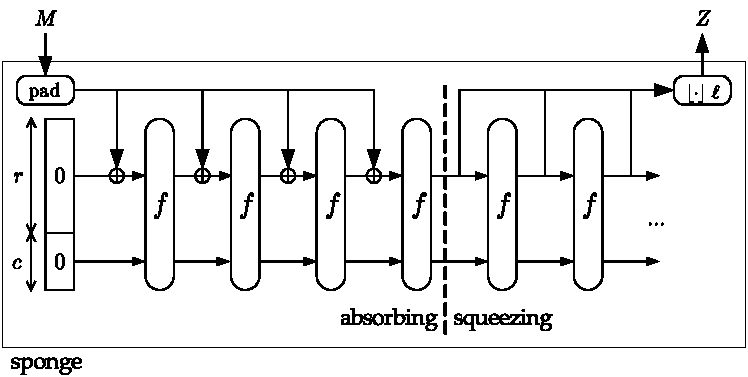
\includegraphics[width=\textwidth]{img/Sponge.pdf}
\caption{The sponge construction $\mathbf{sponge}[f,\mathbf{pad},r]$ \cite{Bertoni2011_SpongeFunctions}}
\label{fig:Sponge}
\end{figure}

The state of the sponge construction is split into two contiguous portions: the \emph{outer state}, which is accessible externally, and the \emph{inner state}, which is hidden.
The size of the outer state is given by the \emph{rate} $r$ and the size of the inner state is specified by the \emph{capacity} $c$.
The size of the entire state is $b = r + c$.
The speed of the construction partially relies on the rate, while the security is partially dependent on the capacity (see Section~\ref{subsec:SpongeSecurity}).

The padding function $\mathbf{pad}$ is first applied to $M$ to make it a multiple of $r$.
$M$ is then absorbed $r$ bits at a time.
More concretely, absorption is the process of XORing $r$-bit blocks into the state while interleaving with applications of the underlying sponge function $f$.
If the rate is increased, then more bits are absorbed at a time and thus the construction runs faster.
However, increasing the rate means that the capacity must decrease and so there is a clear trade-off between speed and security.
Squeezing consists of concatenating $r$ bits at a time to an output bitstring $Z$ that is truncated to $\ell$ bits.
The sponge function $f$ must be called once for each $r$ bits of output after the first full block.

\subsubsection{Simplified Sponge}
A padding function is required for the classical sponge construction in order to ensure that inputs can be reformed into bitstrings with length equal to a multiple of $r$. 
Two basic requirements of a padding function are that it be reversible and that it never produce identical outputs for different inputs.
We omit the lower level details of good padding functions here for brevity and refer the interested reader to \cite{Bertoni2011_SpongeFunctions} instead.

It is also useful, as we will see, to consider a sponge construction in which no padding function $\mathbf{pad}$ is required.
The parameterized interface for such a construction becomes
\begin{equation*}
Z = \mathbf{sponge}[f,r](M,\ell).
\end{equation*}
Alternatively, we can say that $\mathbf{pad}$ exists but it is trivially given as
\begin{equation*}
\mathbf{pad}(M) = M.
\end{equation*}
This lets us remain aligned with the original definition.
In either case, we assume that any necessary padding is performed at some higher level in the overall system.
This simplification allows us to focus more design effort towards the underlying sponge function $f$ and ignore the details of padding.

%For a more concrete treatment, we refer to the official SHA-3 hashing parameters:
\subsection{Applications}
\label{sec:SpongeApplications}
\subsubsection{Hashing}
The sponge construction was originally envisioned as a generalization of hash functions to functions with arbitrary length output.
Using the sponge construction for hashing is straightforward.
We denote a hash function by
\begin{equation*}
\mathbf{H} \from \Ztwo^* \to \Ztwo^{\ell}, 
\end{equation*}
where $\ell$ is the desired length of the message digest.
In this case, the message $M$ is padded and absorbed as usual.
After absorption completes, the construction switches to squeezing mode and the state is squeezed until a message digest of length $\ell$ is acquired.

Without any structural changes, several other applications can be derived from the sponge construction.
These following applications are of considerable relevance to the ultimate goal of authenticated encryption.

\subsubsection{MAC Generation}
A Message Authentication Code (MAC) function is essentially a keyed hash function.
We denote a MAC function under a given key $K$ and initialization vector $IV$ by
\begin{equation*}
\mathbf{MAC}_{K,IV} \from \Ztwo^k \times \Ztwo^v \times \Ztwo^* \to \Ztwo^{\ell},
\end{equation*}
where $k$ is the length of the key, $v$ is the length of the IV, and $\ell$ is the desired length of the tag (MAC).
In this case, $K||IV$ is absorbed first and then the padded message is absorbed directly after as usual.
Squeezing works the same as in a hash computation.
Note that the sponge construction is particularly attractive here (and in general with keyed modes) because to the sponge, there is no differentiation between the key, IV, and message data.
All input data is treated exactly the same, and thus the design remains simple.
This is in great contrast to traditional symmetric key cryptosystem design in which a key schedule is required.

\subsubsection{Bitstream Encryption}
The previous two direct applications of the sponge construction were characterized by long absorbing phases (assuming a long message) and short squeezing phases.
Bitstream encryption, i.e.\ using the sponge as a stream cipher, is characterized oppositely: absorbing is quick while squeezing is likely a much longer process.
We denote a stream cipher under a given key $K$ and initialization vector $IV$ by
\begin{equation*}
\mathbf{STREAM}_{K,IV} \from \Ztwo^k \times \Ztwo^v \to \Ztwo^{\infty},
\end{equation*}
where $k$ is the length of the key and $v$ is the length of the IV.
The codomain of such a stream cipher is the set of infinite bitstreams; in practice, the output is truncated to provide just enough keystream material to encrypt a given message $M$.
For this application, we simply absorb $K||IV$ and switch to the squeezing phase immediately.
Squeezing continues until a keystream is no longer needed.
The keystream is XORed with the message to produce the ciphertext.
Notice again how the overall structure of the algorithm remains the same as it was for its original application of hashing.

\subsection{Generic Security}
\label{subsec:SpongeSecurity}
It is typical to employ Kerckhoffs' principle when discussion the security of a cryptosystem.
This principle states that a cryptosystem should be secure regardless of any knowledge the adversary may have about the system (excluding the key).
Stated in a different way, the adversary is assumed to know every detail of the system except for the key \cite{Stinson2006_CTAP}.
Indeed, we even presume that an attacker has access to the cryptosystem.
In the case of a sponge construction, the adversary knows $f$ (and $f^{-1}$ if $f$ is a permutation).
The easiest way for him or her to gain knowledge about $f$ that may differentiate it from a random transformation is to simply make calls to it (and $f^{-1}$ if a permutation) \cite{Bertoni2011_SpongeFunctions}.

A \emph{random oracle} model is often useful as a framework for security proofs.
A random oracle (RO), which lies at the core of most sponge security proofs, is a theoretical ideal function
\begin{equation*}
\mathbf{RO} \from \mathbb{Z}_2^* \to \mathbb{Z}_2^{\infty}
\end{equation*}
such that every bit of the output, for every possible input, is chosen uniformly and independently. 
We state security proofs in the context of \emph{indistinguishability} in the random oracle model. 
We suppose that an adversary is able to query both a random oracle and the pseudorandom function (PRF) that we are testing.
The adversary then decides which of the systems is the PRF.
If it is ``hard'' for the adversary to do this, then the PRF is called indistinguishable from random. This is what we desire.
Hardness is given in terms of computational complexity and is subject to interpretation.
For example, if the adversary is able to accurately distinguish the two systems after only $2^{40}$ queries, then the PRF is not indistinguishable from random since a complexity of $2^{40}$ is computable with today's technology.
If, however, it takes a minimum of $2^{128}$ queries, then the system \emph{is} indistinguishable from random since this is not computable (i.e.\ such a computation would not finish within any reasonable time frame) and will not be computable in the foreseeable future \cite{Stinson2006_CTAP}.

The security of the sponge construction is based on the assumption that the underlying sponge function $f$ is secure.
That is, if $f$ is indistinguishable from random then so should be the sponge construction it is instantiated within.
Consequently, cryptographers designing a system based on the sponge construction need only be concerned with designing and cryptanalyzing a secure underlying function.
The sponge construction, when used properly, is said to be secure against \emph{generic attacks} -- attacks which do not exploit any specific properties of the underlying sponge function.
We call this the \emph{generic security} of the construction \cite{Bertoni2011_SpongeFunctions}.

\subsection{Security of Keyed Sponges}
The generic security of keyed constructions is higher than unkeyed.
For our purposes we are interested only in the security of the keyed sponge construction where a permutation is used for $f$. 

In \cite{Bertoni2011_SpongeKeyed} it is proven that the \emph{advantage} of distinguishing a keyed permutation-based sponge from a random oracle is
\begin{equation*}
\mathrm{max}\left( 
  1 - \mathrm{exp}\left(
    -\frac{\frac{M^2}{2}+2MN}{2^c}
  \right),
  \frac{N}{2^{|K|}}
\right),
\end{equation*}
where $M$ is the data complexity, $N$ is the time complexity, $c$ is the capacity, and $|K|$ is the size of the key.
The advantage is the probability of success of a generic attack.

We can take $N$ as the number of queries to the permutation $f$ and its inverse.
The data complexity $M$ is typically considered to be upper bounded by the implementation under a given key $K$.
For example, it is very reasonable and common practice to enforce that no more than, say, $M = 2^{40}$ operations be performed under a given key.
In \cite{Bertoni2011_SpongeKeyed} this exponent is called a \emph{usage exponent} and is denoted as $a$.
The assumption is made that $a \ll c / 2$ and the requirement (as is typical) is that no attacks are faster than a brute force search on the keyspace.
This ultimately leads to our metric of interest: a lower bound on the capacity $c$ such that there are no generic attacks (that allow differentiation from a random oracle) that are faster than exhausitive search.
This lower bound is given as
\begin{equation*} 
c \ge |K| + a + 1.
\end{equation*}

Jovanovic et.~al\ \cite{Jovanovic2014_Beyond} further improved on these results in 2014 by proving that the generic security level of keyed sponge constructions is lower bounded by 
\begin{equation*}
\mathrm{min}(2^{(r+c)/2}, 2^c, 2^{|K|}).
\end{equation*} 

%------------------------------
% SECTION:Duplex Construction
%------------------------------
\section{Duplex Construction}
The duplex construction is highly related to the sponge construction.
The main differences are that the duplex construction maintains state between calls and that there no longer exists a clear separation between the absorbing and squeezing phases.
Absorbing and squeezing happen essentially at the same time, hence ``duplexing''.
Other than this, switching from the sponge to the duplex construction is simply a matter of adjusting how inputs and outputs are handled.
The duplex mode has several applications, with authenticated encryption being the one of obvious interest to us.

\subsection{Duplex Parameters}
\begin{figure}[ht]
\centering
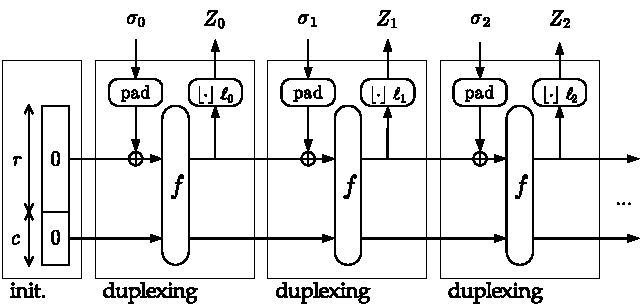
\includegraphics[width=\textwidth]{img/Duplex.pdf}
\caption{The duplex construction $\mathbf{duplex}[f,\mathbf{pad},r]$ \cite{Bertoni2011_SpongeFunctions}}
\label{fig:Duplex}
\end{figure}

Parameters for the duplex construction are mostly the same as for the sponge construction.
However, since the duplex construction maintains state, we build a \emph{duplex object} $D$ and make calls to it.
The function which processes inputs and produces outputs is called $\mathbf{duplexing}$:
\begin{equation*}
Z_i = D.\mathbf{duplexing}(\sigma_i,\ell_i)
\end{equation*}

Figure~\ref{fig:Duplex} shows the duplex construction.
The $i$-th input is denoted $\sigma_i$ and the $i$-th output is denoted $Z_i$, which is truncated to $\ell_i$ bits.
Inputs are absorbed and processed at the same time that outputs are squeezed.
For a duplex object it is possible to have an empty input or to not request an output.
A \emph{blank call} is a call to $\mathbf{duplexing}$ for which no input is provided ($|\sigma_i| = 0$).
A \emph{mute call} is a call for which no output is requested ($\ell_i = 0$).
The reasons for these types of calls will soon be apparent.

\subsubsection{Simplified Duplex}
In addition to the padding required for the sponge construction, the duplex construction also requires \emph{domain separation}.
This can be generally defined as a mechanism that allows differentiation between varying types of inputs (e.g.\ between header and body data).
In other words, it eliminates ambiguity on the receiving end that naturally arises from support for arbitrary length inputs.
The \Keccak designers use a \emph{frame bit} appended to the end of every input (see Figure~\ref{fig:DuplexAE}) in their original definition of the duplex construction \cite{Bertoni2012_Duplexing}.
The value of this bit toggles for every input type so that the receiver can differentiate between outputs.
Since the order of the inputs (and thus outputs) is always the same, a single frame bit is sufficient.

We also note that a frame bit is not the only way to achieve domain separation.
In general one can append a \emph{frame string}, denoted $\gamma_i$, to the end of every input.
The only requirements are that $|\gamma_i| \ge 1$ and $\gamma_i \ne \gamma_{i+1}$ for all $i$. 
For example, each frame string could be a byte instead of a single bit.

For the simplified duplex construction, we can make the assumption that both the padding and domain separation are accomplished at some higher level if needed.
This again allows us to focus more design effort towards the underlying sponge function.

\subsection{Duplex for Authenticated Encryption}
Authenticated encryption is easily achieved using the duplex construction.
It can be modeled under a given key $K$ as
\begin{equation*}
\mathbf{AE}_K \from \mathbb{Z}_2^k \times (\mathbb{Z}_2^*)^2 \to \mathbb{Z}_2^* \times \mathbb{Z}_2^{\ell},
\end{equation*}
where $k$ is the length of the key and $\ell$ is the length of the MAC desired.

Figure~\ref{fig:DuplexAE} shows the duplex construction being used in an AE use case.
Frame bits are shown, but recall that these are ignored in the simplified duplex construction.
First, we construct a duplex object $D$.
Then we absorb $K$ (or optionally $K||IV$) using one or more mute calls to $D.\mathbf{duplexing}$.
More that one mute call may be required if the length of the key exceeds the rate $r$.
We denote a header input to $D$ as $A$; these arbitrary length inputs are authenticated but not encrypted.
We denote a body input to $D$ as $B$; these arbitrary length inputs are both encrypted and authenticated.
$A$ inputs are absorbed using one or more mute calls to $D.\mathbf{duplexing}$.
$B$ inputs are absorbed in a similar fashion and then the keystream $Z$ is XORed with $B$ to produce the ciphertext $C$.
The tag $T$ is produced using a blank call to $D.\mathbf{duplexing}$ after all header and body inputs have been processed.

\begin{figure}[ht]
\centering
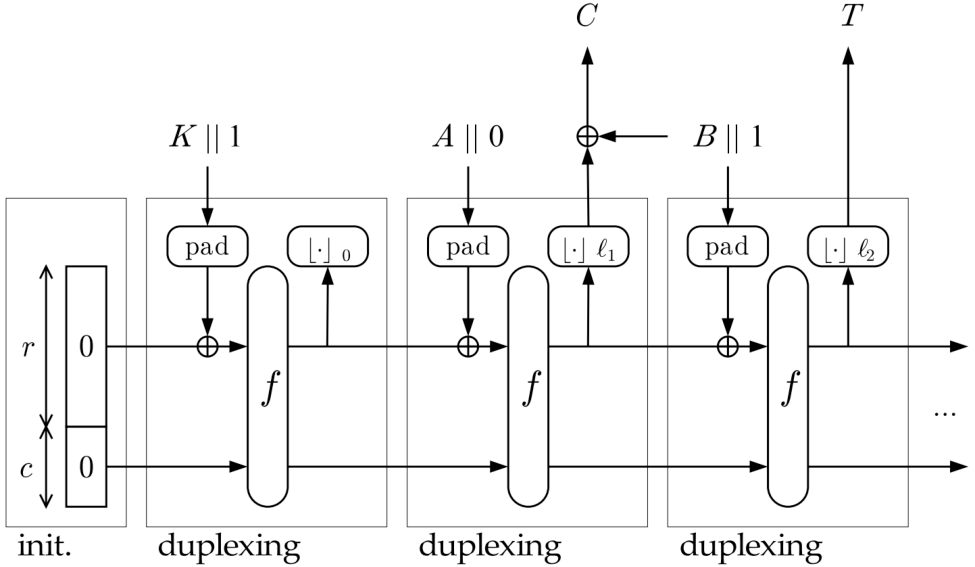
\includegraphics[width=\textwidth]{img/DuplexAE.pdf}
\caption{The duplex construction as used for authenticated encryption \cite{Bertoni2010_DuplexingSlides}}
\label{fig:DuplexAE}
\end{figure}

A more general case is shown in a slightly modified view in Figure~\ref{fig:DuplexAE_Expanded}. 
In this view, the duplex object $D$ is shown as a block and the different header and body inputs ($A_i$ and $B_i$ respectively) are absorbed over a series of calls to $D.\mathbf{duplexing}$. 
For example, the body $B$ consists of three blocks of size $r$ and so it requires three calls to be completely absorbed.
An intermediate tag is requested after the first header and body pair is processed and before the next header begins.
This is a very typical use case for e.g.\ network traffic.
The tag can be of arbitrary length.

\begin{figure}[ht]
\centering
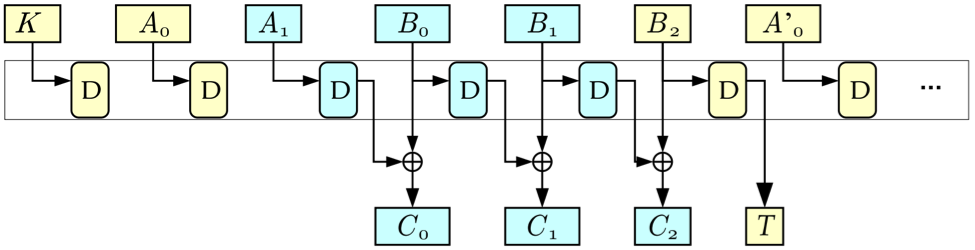
\includegraphics[width=\textwidth]{img/DuplexAE_Expanded.png}
\caption{The duplex construction as used for authenticated encryption (general case) \cite{Bertoni2010_DuplexingSlides}}
\label{fig:DuplexAE_Expanded}
\end{figure}

Clearly, the ciphertext and tags produced at any point depend on all of the previous inputs to $D$.
Intermediate tags can be produced if desired, since blank calls can be made at any time.
In summary, using the duplex construction for authenticated encryption provides the following advantages:
\begin{enumerate}
\item Easy to use
\item Single key required
\item Single-pass for encryption and authentication
\item Support for intermediate tags
\item Support for Additional Authenticated Data (AAD, or headers)
\item Secure against generic attacks
\item Ability to trade off speed and security by adjusting $r$
\end{enumerate}
The main disadvantage to using the duplex construction for AE is that it is not easily parallelizable as given here.
This should not be a concern most of the time since data (e.g.\ IP traffic) is often received and sent in a serial fashion for AE applications.
Compared to other methods of achieving AE, the duplex construction is clearly superior in the majority of applications.

\subsection{Security}
\label{sec:DuplexSecurity}
A reduction is used to prove the security of the duplex construction.
Any calls made to the duplex construction can be reduced to calls to the keyed sponge construction.
Therefore the security of the duplex depends on the security of the corresponding sponge, which can be shown to be secure against generic attacks.
For a concrete example, consider the $i$-th duplexing call to a duplex object $D$:
\begin{align*}
Z_i &= D.\mathbf{duplexing}(\sigma_i,\ell_i) \\
&= \mathbf{sponge}(\mathbf{pad}(\sigma_0)\ ||\ \mathbf{pad}(\sigma_1)\ ||\ \dots\ ||\ \mathbf{pad}(\sigma_i))
\end{align*}
Or in the case of a simplified duplex object $D$, we have:
\begin{align*}
Z_i &= D.\mathbf{duplexing}(\sigma_i,\ell_i) \\
&= \mathbf{sponge}(\sigma_0\ ||\ \sigma_1\ ||\ \dots\ ||\ \sigma_i),
\end{align*}
where $\sigma_i$ may be key, header, or body material.
Since this is true in general, it is clear that the duplex reduces to the sponge.
For a more rigorous proof, we refer to \cite{Bertoni2012_Duplexing}.


%------------------------------
% CHAPTER: Algorithm Specification
%------------------------------
\chapter{Algorithm Specification}
\label{ch:AlgorithmSpec}
Our authenticated encryption algorithm is based on the simplified duplex construction.
Padding and domain separation are assumed to be done at some higher level in the overall system if needed.
For this reason, it is sufficient to specify only the duplex parameters and the sponge function $f$.

For Known Answer Tests (KATs) corresponding to this specification, see Appendix~\ref{appx:KATs}.

\section{Duplex Parameters}
We allow two key sizes: $128$ bits and $256$ bits.
These are the NIST recommended symmetric key sizes as of 2011 \cite{NIST2011_KeySizes}.
Our construction uses a $512$-bit internal state, so we have $b = 512$.
The rate $r$ is $128$ bits for both key lengths, which means that the capacity $c$ is $384$.
Keeping the rate at a constant $128$ bits for both instantiations means that switching between key lengths is a trivial task.

The capacity $c = 384$ provides sufficient security against generic attacks for both $128$- and $256$-bit keys.
As explained in Chapter~\ref{ch:SpongeAndDuplex}, we know from \cite{Jovanovic2014_Beyond} that the generic security level is
\begin{equation*}
\mathrm{min}(2^{(r+c)/2}, 2^c, 2^{|K|}).
\end{equation*}
For a $128$-bit key, the security level is $2^{128}$.
For a $256$-bit key, the security level is $2^{256}$. 

\section{Permutation $f$}
Our underlying sponge function $f$ is a permutation, so it has the advantage of being fully entropy-preserving.
Since it is bijective, $f^{-1}$ exists by definition.
We specify both $f$ and $f^{-1}$ here.
While $f^{-1}$ is never used in practice, it may be useful for cryptanalysis and verification purposes.

\begin{figure}[p,height=.8\textheight]
\centering
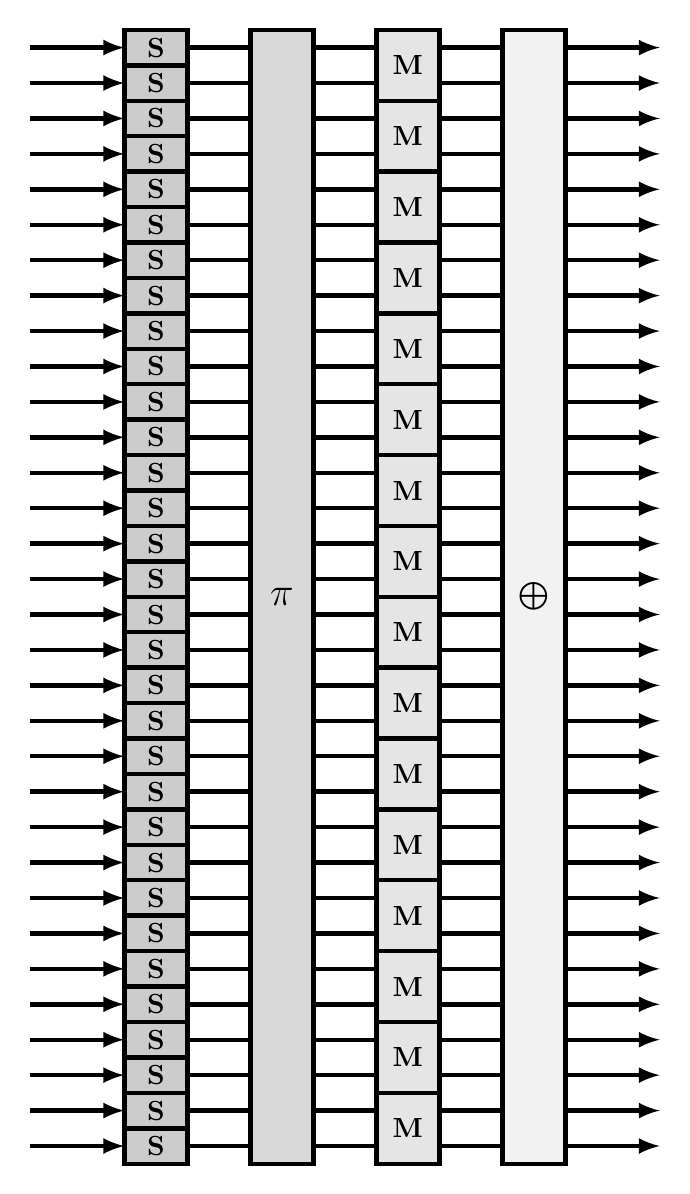
\begin{tikzpicture}[xscale=.8,yscale=0.45,>=latex,ultra thick]
% Reference grid (temporary)
%\draw[help lines] (0,0) grid (16,32);

% TODO label bits / words

% Entry arrows
\foreach \i in {32,...,1} {
  \draw[->] (-1.5,\i-0.5) -- (0,\i-0.5);
}

% Wires
\foreach \j in {1,3,5} {
  \foreach \i in {32,...,1} {
    \draw (\j,\i-0.5) -- (\j+1,\i-0.5);
  }
}

% S-boxes
\foreach \i in {32,...,1} {
  \draw[fill=gray!40] (0,\i) rectangle (1,\i-1) node[midway] {$\mathbf{S}$} ;
}

% P-boxes
\draw[fill=gray!30] (2,0) rectangle (3,32) node[midway] {\Large$\mathbf{\pi}$};

% Mixers
\foreach \i in {32,30,...,2} {
  \draw[fill=gray!20] (4,\i) rectangle (5,\i-2) node[midway] {$\mathbf{M}$};
}

% Round key box
\draw[fill=gray!10] (6,0) rectangle (7,32) node[midway] {$\bigoplus$};

% Exit arrows
\foreach \i in {32,...,1} {
  \draw[->] (7,\i-0.5) -- (8.5,\i-0.5);
}

\end{tikzpicture}


\caption{A single round of the sponge permutation $f$. Each line represents a $16$-bit word.}
\label{fig:Round}
\end{figure}

\begin{figure}[p,height=.8\textheight]
\centering
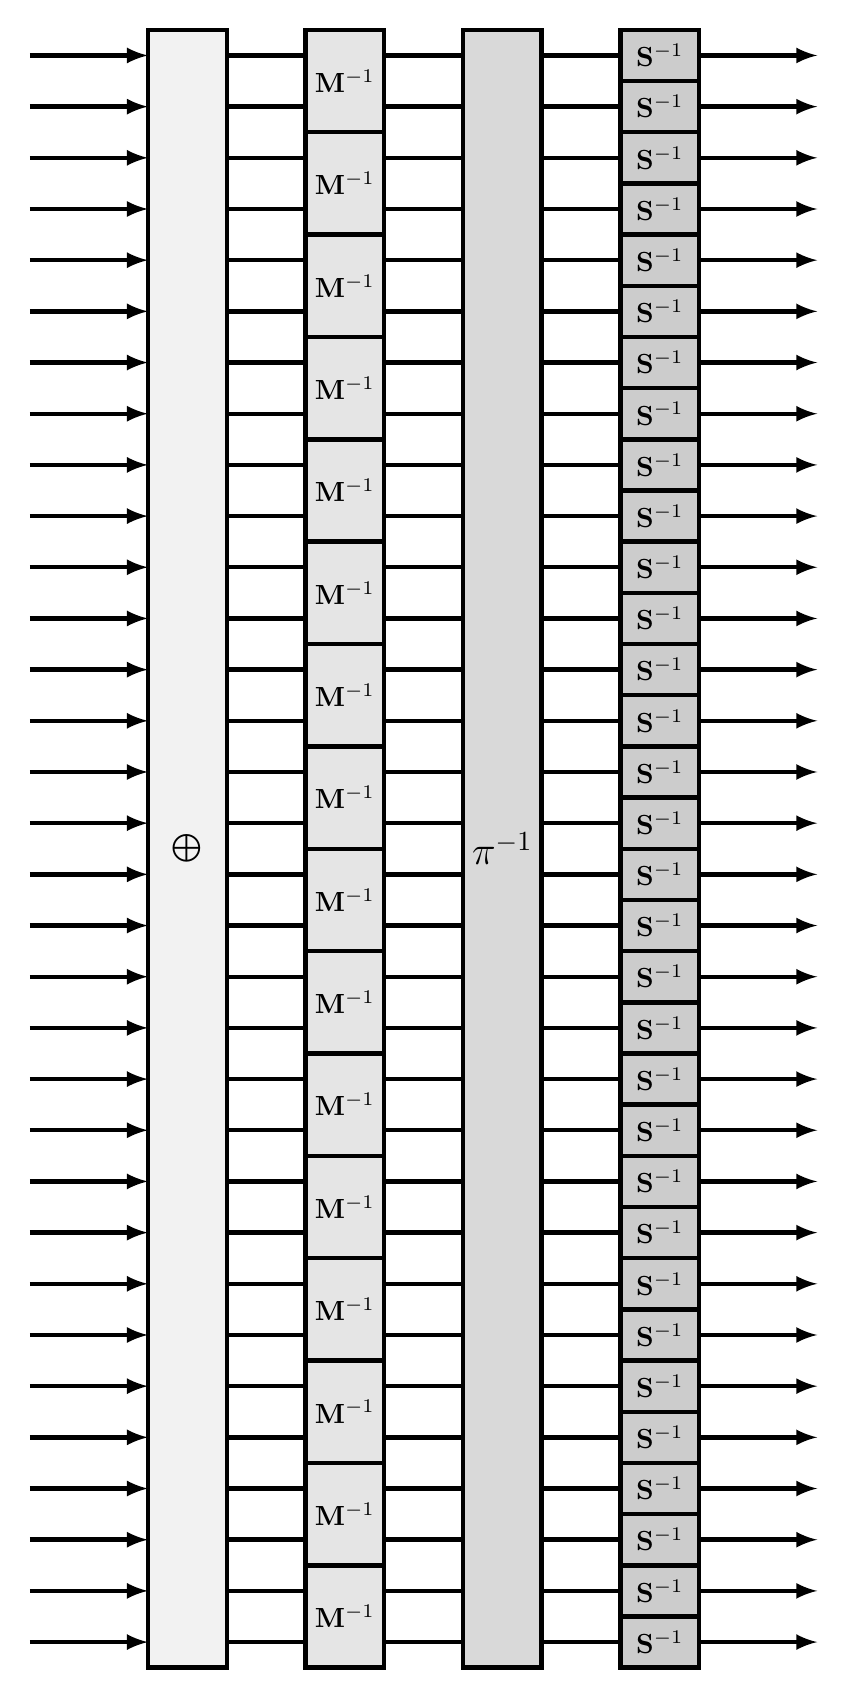
\begin{tikzpicture}[xscale=1,yscale=0.65,>=latex,ultra thick]
% Reference grid (temporary)
%\draw[help lines] (0,0) grid (16,32);

% Entry arrows
\foreach \i in {32,...,1} {
  \draw[->] (-1.5,\i-0.5) -- (0,\i-0.5);
}

% Wires
\foreach \j in {1,3,5} {
  \foreach \i in {32,...,1} {
    \draw (\j,\i-0.5) -- (\j+1,\i-0.5);
  }
}

% Round key box
\draw[fill=gray!10] (0,0) rectangle (1,32) node[midway] {$\bigoplus$};

% Mixers
\foreach \i in {32,30,...,2} {
  \draw[fill=gray!20] (2,\i) rectangle (3,\i-2) node[midway] {$\mathbf{M}^{-1}$};
}

% P-boxes
\draw[fill=gray!30] (4,0) rectangle (5,32) node[midway] {\Large$\mathbf{\pi}^{-1}$};

% S-boxes
\foreach \i in {32,...,1} {
  \draw[fill=gray!40] (6,\i) rectangle (7,\i-1) node[midway] {$\mathbf{S}^{-1}$} ;
}


% Exit arrows
\foreach \i in {32,...,1} {
  \draw[->] (7,\i-0.5) -- (8.5,\i-0.5);
}

\end{tikzpicture}


\caption{An inverse round of the permutation $f$. Each line represents a $16$-bit word.}
\label{fig:RoundInverse}
\end{figure}

The permutation consists of a number of rounds.
Figure~\ref{fig:Round} shows a diagram of a single round of the forward permutation.
Figure~\ref{fig:RoundInverse} shows a single inverse round.
Each round can be represented as the composition of several subfunctions or \emph{steps}: a substitution, a bitwise permutation, a mixing layer, and the addition of a round constant.
These are represented respectively as $\mathbf{S}$, $\mathbf{\pi}$, $\mathbf{M}$, and $\oplus$ in the diagrams.

\subsection{Substitution Step}
The substitution step is a bricklayer permutation that uses $32$ identical, bijective $16 \times 16$ S-boxes.
This step is the main source of confusion within the permutation.
Furthermore, it is the only nonlinear step, as is typical with most substitution-based symmetric key algorithms \cite{Stinson2006_CTAP}.

To the best of our knowledge this is the first cryptosytem to use such large S-boxes.
We believe that, at the time of writing, the largest S-boxes used in the literature are the $8 \times 8$ bijective S-boxes used by the Advanced Encryption Standard (AES) \cite{Daemen2002_DesignOfRijndael}\cite{NIST2001_FIPS-197}.

Our S-box is an AES-inspired design taken directly from Wood's thesis on the subject \cite{Wood2013_SboxThesis}.
The primary reason for using this particular class of $16$-bit S-boxes is that they are efficiently implementable in hardware.
Rather than being based on a random mapping, they are based on multiplicative inversion in a finite field followed by an affine transformation.
This allows us to implement an actual circuit which performs the operations rather than use the corresponding (and prohibitively large) look-up table.

Specifically, we use the reference C implementation provided in Appendix C of the aforementioned thesis.
This S-box is based on multiplicative inversion in $\gfsixteen / \left\langle p(x) \right\rangle$ where 
\begin{equation*}
p(x) = x^{16} + x^5 + x^3 + x + 1.
\end{equation*}
We represent an input to the S-box (and inverse S-box) as a $16$-bit column vector 
\begin{equation*}
x = 
\begin{pmatrix}
x_{15} & x_{14} & \ldots & x_1 & x_0
\end{pmatrix}^\mathrm{T},
\end{equation*}
where $x_{15}$ is the MSB.
Using this notation, the forward S-box function is given as
\begin{equation*}
\renewcommand{\arraystretch}{0.7} % Make it square
\mathbf{S}(x) = 
\begin{pmatrix}
0 & 0 & 1 & 0 & 0 & 0 & 0 & 1 & 0 & 0 & 1 & 1 & 1 & 1 & 1 & 0 \\
1 & 1 & 0 & 0 & 0 & 0 & 0 & 1 & 0 & 1 & 1 & 0 & 1 & 0 & 1 & 0 \\
1 & 1 & 0 & 0 & 1 & 0 & 1 & 1 & 0 & 1 & 0 & 1 & 0 & 0 & 1 & 1 \\
1 & 1 & 1 & 0 & 0 & 0 & 1 & 0 & 0 & 1 & 1 & 0 & 0 & 0 & 0 & 0 \\

1 & 1 & 0 & 0 & 0 & 1 & 1 & 0 & 0 & 1 & 1 & 1 & 1 & 0 & 1 & 1 \\
0 & 1 & 0 & 0 & 0 & 0 & 1 & 1 & 0 & 1 & 1 & 1 & 1 & 1 & 0 & 1 \\
0 & 0 & 1 & 0 & 1 & 0 & 1 & 0 & 1 & 1 & 0 & 0 & 1 & 1 & 0 & 0 \\
1 & 0 & 1 & 1 & 1 & 0 & 1 & 1 & 0 & 0 & 0 & 1 & 0 & 1 & 1 & 1 \\

0 & 1 & 0 & 0 & 0 & 0 & 0 & 0 & 1 & 0 & 0 & 1 & 1 & 1 & 0 & 1 \\
1 & 0 & 1 & 1 & 0 & 0 & 0 & 1 & 0 & 0 & 1 & 0 & 1 & 0 & 0 & 0 \\
1 & 0 & 1 & 0 & 0 & 1 & 1 & 1 & 0 & 0 & 1 & 1 & 0 & 1 & 0 & 0 \\
1 & 0 & 1 & 1 & 1 & 0 & 1 & 1 & 1 & 1 & 0 & 1 & 1 & 0 & 0 & 1 \\

1 & 0 & 1 & 0 & 0 & 1 & 0 & 1 & 1 & 0 & 0 & 1 & 0 & 0 & 0 & 1 \\
0 & 1 & 0 & 0 & 0 & 1 & 1 & 1 & 1 & 0 & 0 & 0 & 0 & 0 & 0 & 1 \\
1 & 0 & 0 & 0 & 1 & 1 & 0 & 1 & 0 & 1 & 1 & 1 & 1 & 0 & 0 & 0 \\
1 & 1 & 0 & 1 & 0 & 1 & 1 & 0 & 1 & 0 & 0 & 1 & 1 & 0 & 0 & 0 \\
\end{pmatrix}
\begin{pmatrix}
x_{15} \\
x_{14} \\
x_{13} \\
x_{12} \\
x_{11} \\
x_{10} \\
x_{9} \\
x_{8} \\
x_{7} \\
x_{6} \\
x_{5} \\
x_{4} \\
x_{3} \\
x_{2} \\
x_{1} \\
x_{0} \\
\end{pmatrix}
^{-1}
\oplus
\begin{pmatrix}
0 \\
1 \\
0 \\
0 \\
0 \\
1 \\
0 \\
1 \\
1 \\
0 \\
1 \\
1 \\
0 \\
1 \\
1 \\
1 \\
\end{pmatrix}
\end{equation*}
and the inverse is
\begin{equation*}
\renewcommand{\arraystretch}{0.7} % Make it square
\mathbf{S}^{-1}(x) = 
\left[
\begin{pmatrix}
0 & 1 & 0 & 1 & 0 & 1 & 1 & 1 & 0 & 0 & 1 & 0 & 0 & 0 & 0 & 1 \\
1 & 1 & 0 & 1 & 0 & 0 & 1 & 0 & 1 & 0 & 1 & 1 & 1 & 1 & 0 & 1 \\
1 & 0 & 1 & 1 & 1 & 1 & 0 & 1 & 0 & 1 & 1 & 0 & 0 & 0 & 0 & 0 \\
0 & 0 & 1 & 0 & 1 & 1 & 1 & 0 & 1 & 0 & 1 & 1 & 1 & 0 & 1 & 0 \\

1 & 1 & 1 & 1 & 1 & 0 & 0 & 0 & 1 & 0 & 0 & 0 & 0 & 1 & 0 & 0 \\
0 & 0 & 0 & 1 & 0 & 1 & 0 & 0 & 0 & 0 & 1 & 1 & 1 & 1 & 1 & 1 \\
1 & 0 & 1 & 0 & 0 & 0 & 0 & 0 & 0 & 1 & 1 & 0 & 1 & 0 & 1 & 1 \\
0 & 0 & 1 & 0 & 1 & 1 & 1 & 0 & 0 & 1 & 0 & 1 & 1 & 1 & 1 & 0 \\

0 & 0 & 0 & 0 & 0 & 0 & 1 & 0 & 0 & 0 & 1 & 0 & 0 & 0 & 1 & 0 \\
1 & 1 & 1 & 0 & 0 & 1 & 1 & 1 & 1 & 0 & 1 & 1 & 1 & 0 & 0 & 0 \\
0 & 1 & 1 & 0 & 1 & 1 & 1 & 1 & 0 & 0 & 1 & 0 & 1 & 1 & 1 & 1 \\
1 & 0 & 0 & 1 & 1 & 0 & 0 & 0 & 1 & 0 & 0 & 1 & 1 & 0 & 1 & 1 \\

1 & 0 & 0 & 0 & 0 & 1 & 0 & 1 & 1 & 1 & 0 & 0 & 1 & 0 & 1 & 0 \\
1 & 0 & 0 & 0 & 0 & 1 & 1 & 1 & 1 & 1 & 0 & 1 & 1 & 1 & 1 & 1 \\
1 & 1 & 1 & 0 & 0 & 1 & 1 & 0 & 1 & 0 & 0 & 1 & 1 & 1 & 1 & 1 \\
0 & 1 & 0 & 0 & 1 & 0 & 1 & 0 & 1 & 0 & 0 & 1 & 0 & 0 & 0 & 1 \\
\end{pmatrix}
\begin{pmatrix}
x_{15} \\
x_{14} \oplus 1 \\
x_{13} \\
x_{12} \\
x_{11} \\
x_{10} \oplus 1 \\
x_{9} \\
x_{8} \oplus 1 \\
x_{7} \oplus 1 \\
x_{6} \\
x_{5} \oplus 1 \\
x_{4} \oplus 1 \\
x_{3} \\
x_{2} \oplus 1 \\
x_{1} \oplus 1 \\
x_{0} \oplus 1 \\
\end{pmatrix}
\right]^{-1}.
\end{equation*}

A hardware implementation for this particular S-box requires just $1238$ XOR gates and $144$ AND gates.
However, No concrete implementation (e.g.\ in VHDL) is provided; this is an area for future work.

\subsection{Bitwise Permutation Step}
Bitwise permutations are easily implementable in hardware via a simple rerouting of wires.
Compared to a permutation on the words of the state, a bitwise permutation intuitively provides much better diffusion.
The bitwise permutation step is the main source of long-range (i.e.\ across the entire state) diffusion in the algorithm.

The bitwise permutation also helps maximize the minimum number of active S-boxes by being subject to certain constraints.
We use a permutation that satisfies the following properties:
\begin{enumerate}
\item All outputs of a given S-box go to $16$ different mixers
\item The permutation is a \emph{derangement}; it has no fixed points
\item High order; it does not repeat within the number of rounds
\item No low order bits; the order of any bit equals the order of the overall permutation
\item Easily definable by some function
\end{enumerate}
There is obviously no cryptographic significance to how ``easy'' it is to express a bitwise permutation.
This is merely to cut down on the search space and to avoid having to provide a table with $512$ entries to express the permutation.

We denote the bitwise permutation function
\begin{equation*}
\pi \from \mathbb{Z}_{512} \to \mathbb{Z}_{512},
\end{equation*}
where it operates on the \emph{index} of a given bit, $x \in \mathbb{Z}_{512}$. 

To understand our specific choice of $\pi$, it is useful to consider a poor choice first.
For this we can turn our attention to the lightweight block cipher PRESENT which operates on a $64$-bit state over $31$ rounds.
PRESENT uses the bitwise permutation
\begin{equation*}
\pi_P \from \mathbb{Z}_{63} \to \mathbb{Z}_{63}
\end{equation*}
given by the linear function
\begin{equation*}
\pi_P(x) = 16x \bmod{63}.
\end{equation*}
Since it operates in $Z_{63}$, an augmented mapping $\pi_P(63) = 63$ is required for the last bit \cite{Bogdanov2007_PRESENT}.

The particular structure of $\pi_P$ led to an attack on PRESENT in 2009 \cite{Nakahara2009_PRESENT_Cryptanalysis}.
The attack leverages the following undesirable properties of $\pi_P$:
\begin{enumerate}
\item There are four fixed points: $x = 0, 21, 41, 63$
\item The order is only three: $\pi_P^3(x) = \pi_P(x)$
\end{enumerate}
The combination of these properties results in a decrease in the lower bound on the number of active S-boxes across four rounds since it is possible to construct a trail that branches back into itself after $\pi_P$ is iterated only three times.
See Figure~\ref{fig:PRESENT_Trail} for a diagram that illustrates this trail.

A simple way to avoid fixed points is to use an affine function rather than a linear function.
An affine function over $\mathbb{Z}_{512}$ is of the form
\begin{equation*}
\pi(x) = \alpha x + \beta \bmod{512}.
\end{equation*}
For $\pi$ to be bijective, we require $\gcd(\alpha, 512) = 1$.
Since the prime factorization of $512$ is simply $2^9$, it is equivalent to say that $\alpha$ must be odd \cite{Stinson2006_CTAP}.

A low order bit is defined as a bit that has order less than the order of the overall bitwise permutation.
It is cumbersome to mathematically characterize all permutations that satisfy the property that no bits have low order. Instead, we wrote a script (see Appendix~\ref{appx:SourceCodeListings}) to search for such permutations.
The script also identifies if a given permutation satisfies all other properties that we require.
We found $384$ permutations defined by affine functions over $Z_{512}$ that satisfy all properties. A complete listing is provided in Table~\ref{tab:BitwisePermutations}.

We chose the following permutation to use for our algorithm since it is the first function to satisfy all properties:
\begin{equation*}
\pi(x) = 31x + 15 \bmod{512}
\end{equation*}
This particular bitwise permutation has order $32$ and its inverse is given by
\begin{equation*}
\pi^{-1}(x) = 479(x-15) \bmod{512}
\end{equation*}
since $31^{-1} \equiv 479$ in $\mathbb{Z}_{512}$.

\subsection{Mix Step}
The purpose of the mix step is to provide local diffusion (i.e.\ across two words) and increase the linear and differential branch numbers of a round from two to three.
See Chapter~\ref{ch:Cryptanalysis} for more detail on branch numbers.
We use a mixer based on multiplication by a $2 \times 2$ matrix in \gfsixteen modulo the irreducible polynomial
\begin{equation*}
p(x) = x^{16} + x^5 + x^3 + x^2 + 1.
\end{equation*}
The mixer takes two words $A$ and $B$ as input and produces outputs $A'$ and $B'$ as follows:
\begin{equation*}
\begin{pmatrix}
A' \\ B'
\end{pmatrix}
=
\begin{pmatrix}
1 & x \\ x & x + 1
\end{pmatrix}
\begin{pmatrix}
A \\ B
\end{pmatrix}
\end{equation*}
The mix step is invertible because the matrix is invertible; its inverse is given by
\begin{equation*}
\begin{pmatrix}
A \\ B
\end{pmatrix}
=
\begin{pmatrix}
a & b \\ b & c
\end{pmatrix}
\begin{pmatrix}
A' \\ B'
\end{pmatrix}
\end{equation*}
where
\begin{align*}
a &= x^{15} + x^{14} + x^{12} + x^{11} + x^9 + x^8 + x^6 + x^5 + x^4 + x + 1 \\
b &= x^{14} + x^{13} + x^{11} + x^{10} + x^8 + x^7 + x^5 + x^4 + x^3 + 1 \\
c &= x^{15} + x^{13} + x^{12} + x^{10} + x^9 + x^7 + x^6 + x^3 + x.
\end{align*}
This can be verified by using the provided \gfsixteen C library.
The MSB of each word is taken as the leftmost bit and is represented by $x^{15}$. 

The forward mixer is efficiently implementable in hardware.
Notice that the outputs $A'$ and $B'$ can be written as
\begin{align*}
A' &= A \oplus Bx \\
B' &= Ax \oplus Bx \oplus B
\end{align*}
since addition in \gfsixteen is simply the XOR operation.
Figure~\ref{fig:MixerMatrix} shows how this matrix multiplication is implemented.

\begin{figure}[ht]
\centering
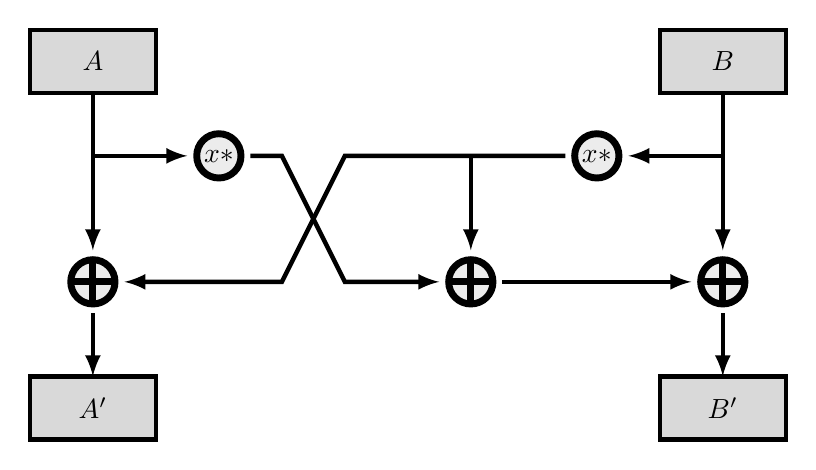
\begin{tikzpicture}[xscale=0.8,yscale=0.8,>=latex,ultra thick]
% Reference grid (temporary)
%\draw[help lines] (0,0) grid (16,16);

% Inputs
\draw[fill=gray!30] (0,15) rectangle (2,14) node[midway] {$A$};
\draw[fill=gray!30] (10,15) rectangle (12,14) node[midway] {$B$};

\draw[->] (1,14) to (1, 11.5);
\draw[->] (1,13) to (2.5, 13);

\draw[->] (11,14) to (11, 11.5);
\draw[->] (11,13) to (9.5, 13); 

\drawxTimes{3}{13}
\drawxTimes{9}{13}

\drawXOR{1}{11}
\drawXOR{11}{11}
\drawXOR{7}{11}

\draw[->] (3.5,13) to (4,13) to (5,11) to (6.5,11);
\draw[->] (8.5,13) to (5,13) to (4,11) to (1.5,11); 
\draw[->] (7,13) to (7,11.5);
\draw[->] (7.5,11) to (10.5,11);

\draw[->] (1,10.5) to (1,9.5);
\draw[->] (11,10.5) to (11,9.5);

% Outputs
\draw[fill=gray!30] (0,9.5) rectangle (2,8.5) node[midway] {$A'$};
\draw[fill=gray!30] (10,9.5) rectangle (12,8.5) node[midway] {$B'$};

\end{tikzpicture}

\caption{Hardware implementation of the forward mixer function.}
\label{fig:MixerMatrix}
\end{figure}

The $x*$ operation is a multiplication by $x$ in \gfsixteen.
Its implementation, which is shown in Figure~\ref{fig:xTimes}, is very simple. 
Notice that a multiplication by $x$ is simply a left rotation followed by a reduction if the MSB was one.
The reduction is derived from the fact that
\begin{equation*}
x^{16} \equiv x^5 + x^3 + x^2 + 1 \bmod{p(x)}
\end{equation*}
for our particular irreducible polynomial $p(x)$, and it is implementable using just three XOR gates.

\begin{figure}[ht]
\centering
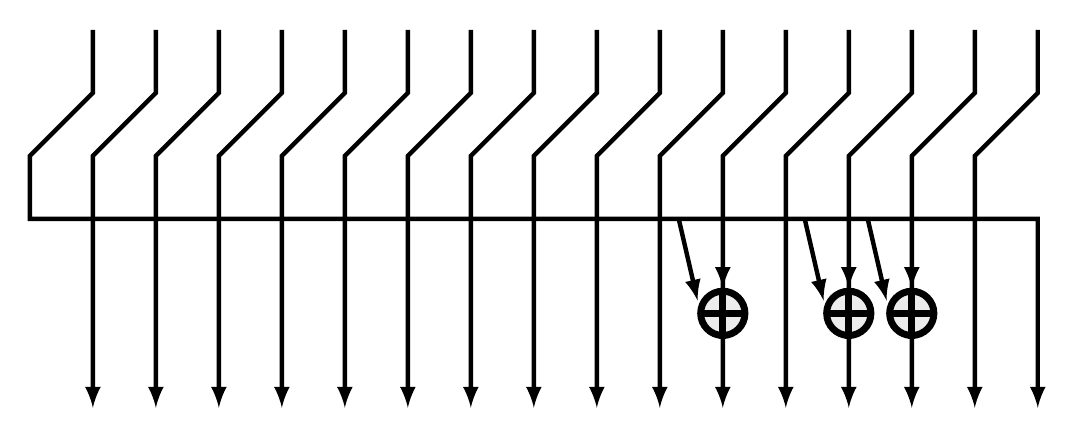
\begin{tikzpicture}[xscale=0.8,yscale=0.8,>=latex,ultra thick]
% Reference grid (temporary)
%\draw[help lines] (0,0) grid (24,24);

\draw[->] (1,24) to (1,23) to (0,22) to (0, 21)
    to (16, 21) to (16, 18);
\foreach \i in {2,...,16} {
    \draw[->] (\i,24) to (\i,23) to (\i-1,22) to (\i-1, 18);
}
\draw[->] (10.3,21) to (10.6,19.7);
\draw[->] (11,21) to (11,19.9);
\drawXOR{11}{19.5}
\draw[->] (12.3,21) to (12.6,19.7);
\draw[->] (13,21) to (13,19.9);
\drawXOR{13}{19.5}
\draw[->] (13.3,21) to (13.6,19.7);
\draw[->] (14,21) to (14,19.9);
\drawXOR{14}{19.5}
\end{tikzpicture}

\caption{Hardware implementation of the $x*$ function. The leftmost bit is the MSB.}
\label{fig:xTimes}
\end{figure}

\subsection{Add Round Constant Step}
The add round constant step is the simplest by far, and it is its own inverse.
A constant $512$-bit value is added to the state using bitwise XOR in order to disrupt symmetry and prevent slide attacks.
The round constant $RC_i$ for round $i$ is given by the formula
\begin{equation*}
RC_i = \mathbf{SHA3\textbf{-}512}(\mathbf{ASCII}(i)),
\end{equation*}
where $\mathbf{ASCII}(i)$ is a function that provides the one or two byte ASCII representation of $i$ and $\mathbf{SHA3\textbf{-}512}$ is the SHA-3 hash function that outputs a $512$-bit message digest. 
Table~\ref{tab:RC} provides the values of $RC_i$ up to $i = 16$.

\makeatletter
\preto{\@verbatim}{\topsep=1em \partopsep=0pt \parskip=0pt \parsep=0pt}
\makeatother

\renewcommand{\arraystretch}{0}

\begin{table}[p]
\begin{tabular}{m{0.1\textwidth}|m{0.8\textwidth}}
\textbf{Constant} & \textbf{Hex Value} \\
& \\

\hline
\centering
$RC_1$ & 
\footnotesize
\begin{verbatim}
00197a4f5f1ff8c356a78f6921b5a6bfbf71df8dbd313fbc5095a55de756bfa1
ea7240695005149294f2a2e419ae251fe2f7dbb67c3bb647c2ac1be05eec7ef9
\end{verbatim}

\\ \hline
\centering
$RC_2$ & 
\footnotesize
\begin{verbatim}
ac3b6998ac9c5e2c7ee8330010a7b0f87ac9dee7ea547d4d8cd00ab7ad1bd5f5
7f80af2ba711a9eb137b4e83b503d24cd7665399a48734d47fff324fb74551e2
\end{verbatim}

\\ \hline
\centering
$RC_3$ & 
\footnotesize
\begin{verbatim}
ce4fd4068e56eb07a6e79d007aed4bc8257e10827c74ee422d82a29b2ce8cb07
9fead81d9df0513bb577f3b6c47843b17c964e7ff8f4198f32027533eaf5bcc1
\end{verbatim}

\\ \hline
\centering
$RC_4$ & 
\footnotesize
\begin{verbatim}
5058cb975975ceff027d1326488912e199b79b916ad90a3fe2fd01508cd7d7c0
1bc8aaa4d21a8473fb15f3b151ab9e44172e9ccb70a5ea04495af3ec03b5153e
\end{verbatim}

\\ \hline
\centering
$RC_5$ & 
\footnotesize
\begin{verbatim}
84da272d13a44f0898ee4ea53334c255d894cc54d357c55466d760debde482a2
44c128df641e80673a8bc34a1620d880b7965e549f313ddccfd506b073413b87
\end{verbatim}

\\ \hline
\centering
$RC_6$ & 
\footnotesize
\begin{verbatim}
bb93aaa23b38ea96c9346ef91e184982bf50e91033f4354ecb20d3c7390c2b41
862e8825ec3d0fee0a6f978881f90728c6748e4aed8b732350075d6c2bdd8e4b
\end{verbatim}

\\ \hline
\centering
$RC_7$ & 
\footnotesize
\begin{verbatim}
fe32f3eba76626dedf36622bfdc5ccd33db2f3e0dd7c3c128298ea78c1cc7fee
1a140edb8e57cd5824c7f4b817c0fc94e70da5b9399faaf9a848a46ad30679e9
\end{verbatim}
  
\\ \hline
\centering
$RC_8$ & 
\footnotesize
\begin{verbatim}
952ba02486b818febc0ec98559df27c79357838f011b1e5bc11f2cfb6fc0573e
545978c2bc5b390f44907f8da0dfd68206fe4521f86ba6c879ec1e69caed9533
\end{verbatim}
  
\\ \hline
\centering
$RC_9$ & 
\footnotesize
\begin{verbatim}
b41e6bb4ed20294016399c268da6bf88c89e2dc118a361b3560ee8daed973a8f
9778df40e308c1206fa42f97f3fd3f63d2b4b3b57eb5bcbec6ad64d46216b692
\end{verbatim}
  
\\ \hline
\centering
$RC_{10}$ & 
\footnotesize
\begin{verbatim}
6954a418cecc43633bd526c2499dfc16b832f58b216b9a8b226a6a0b7918d364
a7939004339de0ba08e2b547e64dc5622e24b0c4f8f415d9e0a84cb94b6c5f3f
\end{verbatim}
  
\\ \hline
\centering
$RC_{11}$ & 
\footnotesize
\begin{verbatim}
2e4b9ad37091e3e5a218c5e57b33ed3470ba4f31fbcf16424684fdd5cde38e88
9eae3f018b37af58c24ccc8af57abc2c6911408dd20ef6435e4494a3e6599a06
\end{verbatim}
  
\\ \hline
\centering
$RC_{12}$ & 
\footnotesize
\begin{verbatim}
aa42aca73bd7f8a17e987f281422b266e44f0de1615d2d393c620c8c5a2c80b4
f06178c8455bf98179603f2f1bcb30b2559f282c799e40533b0665f97a2a706a
\end{verbatim}
  
\\ \hline
\centering
$RC_{13}$ & 
\footnotesize
\begin{verbatim}
969c39ae2dc16834310344c0579d0ffdfde01772dbf9a4cab984953c395d7791
1510f39e5f37295e3611a1d46101460daf731ddbdab1ec1bbc512edc44680d8d
\end{verbatim}
  
\\ \hline
\centering
$RC_{14}$ & 
\footnotesize
\begin{verbatim}
8a1e6ce31f0b526d884b584aa1a5ae4294fcf85fd2e525f959ed1a54233359c7
c5fece6d24775e7d4a9ad97c2632a3be5b331a8f580f557b269e7b65123a5992
\end{verbatim}
  
\\ \hline
\centering
$RC_{15}$ & 
\footnotesize
\begin{verbatim}
9bd64a932f09672def04b6a94753a3e4087a1c3895078dc70927fcd774888dfd
400b95fd1c6a0b2a91a1ba44eea09f5163dba4dfa9da7b8eb97d791cab566437
\end{verbatim}
  
\\ \hline
\centering
$RC_{16}$ & 
\footnotesize
\begin{verbatim}
48401f65c2d2d9e71fe47bd80b28d834eee8fff3be9aa4608cba33e6fedce0b1
693c80cdc36db7f504e4abea23ccc6729a030f5b3e035fb59c2c788215cf84a8
\end{verbatim}

\end{tabular}
\caption{Round constants for up to $16$ rounds}
\label{tab:RC}
\end{table}

\renewcommand{\arraystretch}{1}


\section{Number of Rounds}
This algorithm uses $10$ rounds for a $128$-bit key and $16$ rounds for a $256$-bit key.
The number of rounds is determined, as is typical with block ciphers and permutations, by calculating the number needed for resistance to linear and differential cryptanalysis and adding some buffer to increase the security margin. 
For a more in-depth treatment, refer to Chapter~\ref{ch:Cryptanalysis}.

\section{Customization}
While a specific instantiation is specified here, our algorithm is highly customizable within our security margin.
This could be useful in the case that different users want unique, proprietary algorithms.
We list several possible customizations here.

\subsection{State Initialization}
In the given specification, the inner state (like the outer state) is initialized to zero.
This is not a requirement; indeed, the inner state could be initialized to any $384$-bit value.
Each user could generate their own unique value to set during the initialization phase.
This happens before the first mute calls that absorb the key.

\subsection{S-boxes}
The AES-inspired S-box used here is efficiently implementable in hardware.
There are certainly many other cryptographically secure $16$-bit S-boxes, but randomly generated ones may not be suitable for hardware implementation due to size constraints.
This is an area for further research.
Still, several other AES-like $16$-bit S-boxes are presented in \cite{Wood2013_SboxThesis}.
Any new S-box introduced into the algorithm shall be analyzed to determine its linear and differential characteristics and the number of rounds should be adjusted accordingly if necessary.

\subsection{Bitwise Permutations}
The bitwise permutation provided in the specification is subject to the constraints explained before.
There are many permutations that satisfy these constraints.
We chose to use a permutation that is easily definable by an affine function as obtained by our script; this is not a requirement.
A user could generate their own bitwise permutation subject to the given constraints via exhaustive search.

\subsection{Mixers}
Our mixer is based on a specific $2 \times 2$ matrix multiplication in \gfsixteen modulo a specific irreducible polynomial $p(x)$.
Many matrices are expected to satisfy the constraints that we impose.
These constraints are:
\begin{enumerate}
\item The matrix should be invertible in $\gfsixteen /\left\langle p(x) \right\rangle$
\item The matrix should have differential and linear branch number equal to three (the maximum possible; see Chapter~\ref{ch:Cryptanalysis})
\item The transformation should be efficiently implementable in hardware
\end{enumerate}
Note that the inverse transformation need not be efficiently implementable.
Like the addition of a new S-box, any new mixer (i.e.\ matrix) introduced to the algorithm should be analyzed to ensure it meets these constraints.
A transformation defined by $2 \times 2$ matrix multiplication that does meet the second requirement, for example, would lower our security margin and possibly require increasing the number of rounds significantly.

It should be noted that before settling on a mixer based on matrix multiplication, many mixers based on modular addition, XOR, and rotation operations were tested.
Systems or operations that rely mainly on these operations are typically called \emph{ARX-based}.
None of the ARX-based mixers we tested met our requirement of increasing the branch number from two to three.
However, for completeness, we enumerate all of the mixers examined in this work in Appendix~\ref{appx:ARX_Mixers}.

\subsection{Round Constants}
The round constants presented here are based on SHA-3 hash values.
However, they could be any values that satisfy the following constraints.
Round constants should be:
\begin{enumerate}
\item Unique for each round; to prevent against slide attacks
\item Random, pseudorandom, or highly asymmetric; to reduce symmetry in the state
\end{enumerate}
The round constants are not expected to have any cryptographic significance outside of this.
Different users can generate their own unique set of round constants without difficulty.

There are also other ways of injecting asymmetry into the algorithm using constants.
For example, the round constants could actually be rotation constants that define the amount to rotate each word on the inputs to mixers.


%------------------------------
% CHAPTER: Cryptanalysis
%------------------------------
\chapter{Cryptanalysis}
\label{ch:Cryptanalysis}
We have already discussed the security of this construction against generic attacks in Chapter~\ref{ch:SpongeAndDuplex}.
The only requirement remaining is to assess the security of the underlying sponge permutation $f$.

We present a survey of potentially relevant cryptanalysis techniques here.
Focus is placed on differential and linear cryptanalysis since these techniques are so general, powerful, and prevalent.
Resistance against these techniques should result in resistance against many other less general techniques.
There is far too much to be said about various cryptanalysis techniques, and there are far too many to discuss here.
Our aim is to provide intuitive explanations of prevalent methods and simply explain why our permutation should be resistant.
Further cryptanalysis, as with all cryptosystems, is always welcome for future work.

%------------------------------
% Section: Differential Cryptanalysis
%------------------------------
\section{Differential Cryptanalysis}
Differential cryptanalysis was publicly introduced by Biham and Shamir in 1991 in their landmark paper on the subject, \cite{Biham1991_Differential}.
Since then, it has been applied with varying degrees of success to a great number of cryptosystems.
As such, it is a fundamental requirement of symmetric key cryptosystem design to prove resistance to differential cryptanalysis.

\subsection{Overview}
% XOR is involutive
The goal of differential cryptanalysis is to exploit non-random behavior of a system (in our case, a permutation) with regard to the propagation of differences.
A \emph{difference}, denoted $\Delta X$, is the bitwise XOR (for our case) of two bitstrings. For example,
\begin{equation*}
\Delta X = X' \oplus X''
\end{equation*}
is the difference between bitstrings $X'$ and $X''$.
For differential cryptanalysis, a difference $\Delta X$ is fed through a system and a resulting difference $\Delta Y$ is obtained.
The pair of these two related differences is called a \emph{differential} and is denoted $(\Delta X,\Delta Y)$.

Differentials occur with some associated probability.
For an ideal system the probability of a given differential is $1/2^n$ where $n$ is the length of the bitstrings involved.
A system is said to exhibit non-random behavior if the magnitude of the probability $p_D$ for some differential $(\Delta X, \Delta Y)$ is much greater than the ideal value.
This information could be used to mount an attack on the system \cite{Heys2002_Tutorial}.

To launch an effective attack, a cryptanalyst first has to focus on the S-boxes.
The S-boxes are analyzed to determine their maximum differential probabilities.
Note that in an actual attack, high probability $1$-bit-to-$1$-bit differentials are of most interest since these will likely be the easiest to propagate through the overall system.

A \emph{differential trail} or \emph{characteristic} is the propagation of non-zero differentials throughout a system (i.e.\ across rounds).
Figure~\ref{fig:PRESENT_Trail} shows an example trail through four rounds of PRESENT.
A \emph{differentially active} S-box is an S-box that has a non-zero difference at its input during an attack; it is part of a differential trail.
For example, if Figure~\ref{fig:PRESENT_Trail} shows a differential trail, then there are six differentially active S-boxes.

Proving resistance against differential cryptanalysis for a substitution-permutation network requires coming up with a lower bound on the minimum number of active S-boxes across some number of rounds.
The more active S-boxes there are, the less likely an attack is to succeed since exponentially more chosen plaintexts will be needed for additional each active S-box.
The \emph{branch number} of an operation is of particular importance here. 
It can be simply defined as the minimum number of active S-boxes across just two rounds of a system (e.g.\ our permutation).
The technique of maximizing the branch number of a round is known as the \emph{wide trail design strategy}.
It is the main design strategy behind AES, which has a round branch number of five \cite{Daemen2001_WideTrail}\cite{Daemen2002_DesignOfRijndael}.

The number of plaintext/ciphertext pairs required to mount a successful differential attack should exceed the number required for a brute force attack.
As the differential probability reduces across rounds, more pairs are required for a successful attack.
We loosely refer to the number of pairs required as the \emph{complexity} of the differential attack.
The number of rounds is increased until this complexity exceeds that of a brute force method.

\subsection{Algorithm Resistance}
To determine the resistance of our algorithm to differential cryptanalysis, we first have to determine the maximum differential probability of our S-box.
We determined this value to be $p_{D,max} = 2^{-14}$ using an S-box evaluation program called \texttt{Eval16BitSbox} written with Kaminsky's Parallel Java 2 library \cite{Kaminsky2014_BlockCipherAnalysis}\cite{Kaminsky2014_PJ2}.

Next, it is necessary to determine the branch number of a round.
For this, we only need to analyze the mixer. 
We purposefully designed a mixer with differential branch number equal to three, meaning that minimally three S-boxes will be differentially active between two rounds.
This is in fact the maximum achievable branch number for a transformation defined by multiplication by a $2 \times 2$ matrix.
To verify this, we used a SAT solver called CryptoMiniSat \cite{Soos2014_CryptoMiniSat}.
This SAT solver takes as input a Boolean equation in conjunctive normal form (CNF) and determines if it is \emph{satisfiable}; that is, if it can ever produce an output of `$1$' for any set of input values.
Our CNFs were generated using Kaminsky's \texttt{SatProblem} Java class \cite{Kaminsky2014_BlockCipherAnalysis}.
The Boolean satisfiability problem is known to be NP-complete \cite{Sipser2012_TheoryOfComputation}; however, our CNFs were small enough that it finished within a minute for all cases tried (see Appendix~\ref{appx:ARX_Mixers} for failed mixer designs).

The CNFs generated are unsatisfiable if and only if the mixer has differential branch number equal to three since it answers the following question: \emph{is it possible to have a difference in only one input and only one output?}
Through SAT solver analysis we determined that this is not possible for our matrix multiplication-based mixer; that is, if there is a non-zero difference in only one input, there must be a non-zero difference in each output.
In the event that there is a difference in both inputs, there may be a difference in only one output.
This still leads to a differential branch number of three since two S-boxes must have been active in the previous round to lead to those two input differences.
The probability of a difference in either output is $p_{D,out} = 2^{-15}$.

With all of this information, it is possible to calculate the number of rounds needed for resistance to differential attacks.
The worst-case probability of successfully propagating a difference over two rounds is given by
\begin{equation*}
(p_{D,max})^{\mathcal{B}_D} \cdot p_{D,out},
\end{equation*}
where $\mathcal{B}_D = 3$ is the differential branch number.
From this we constructed Table~\ref{tab:DifferentialProbabilities}, which shows the worst-case differential probabilities for higher numbers of rounds.
\begin{table}[ht]
\centering
\begin{tabular}{c|c}
Rounds & Worse Case Differential Probability \\
\hline
$2$  & $2^{-57}$  \\
$4$  & $2^{-114}$ \\
$6$  & $2^{-171}$ \\
$8$  & $2^{-228}$ \\
$10$ & $2^{-285}$ \\
$12$ & $2^{-342}$ \\
$14$ & $2^{-399}$ \\
$16$ & $2^{-456}$ \\
\end{tabular}
\caption{Worst case differential probabilities over increasing rounds}
\label{tab:DifferentialProbabilities}
\end{table}

Therefore the complexity of a differential attack exceeds the complexity of a brute force search of a $128$-bit keyspace at six rounds.
To increase our security margin significantly, we require $10$ rounds for a $128$-bit key.
For a $256$-bit key, $16$ rounds are required to achieve a similar security margin.

%------------------------------
% Section: Linear Cryptanalysis
%------------------------------
\section{Linear Cryptanalysis}
Linear Cryptanalysis was first introduced by Matsui in 1993 in his landmark paper, \cite{Matsui1993_Linear}.
As with differential cryptanalysis, it is a fundamental requirement of symmetric key cryptosystem design to prove resistance against linear attacks.

\subsection{Overview}
Linear cryptanalysis is surprisingly similar to differential cryptanalysis in many ways. 
However, for linear cryptanalysis we are concerned with estimating the behavior of a system using linear expressions rather than highly probable differential characteristics.
As with differential cryptanalysis, the first step is to analyze the S-boxes involved in the substitution-permutation network.
An S-box, by definition, should be highly nonlinear to provide sufficient confusion. 
However, it is possible to uncover linear approximations of S-box outputs that occur with high (or low) probability.
We can represent our S-box as a vectorial Boolean function 
\begin{equation*}
S \from \Ztwo^{16} \to \Ztwo^{16}
\end{equation*}
in which the input $X$ and output $Y$ are represented as row vectors, e.g.\
\begin{equation*}
X = \begin{pmatrix}X_1 & X_2 & ... & X_{15} & X_{16} \end{pmatrix},
\end{equation*}
where $X_i \in \Ztwo$.
Favoring typical convention found in the literature, $X_1$ is the MSB \cite{Heys2002_Tutorial}.
This notation allows us to easily represent linear approximations in the form
\begin{equation*}
\left( \bigoplus\limits_{i=1}^{16} X_i \right) = \left( \bigoplus\limits_{i=1}^{16} Y_i \right)
\end{equation*}
or equivalently
\begin{equation*}
\left( \bigoplus\limits_{i=1}^{16} X_i \right) \oplus \left( \bigoplus\limits_{j=1}^{16} Y_j \right) = 0.
\end{equation*}

The ideal \emph{linear probability} $p$ that such an approximation holds true is exactly equal to 1/2.
We are concerned with deviations from this ideal probability, known as the \emph{linear bias}, $\epsilon$. 
Clearly, $\epsilon = p - 1/2$.
We found the maximum linear bias of our particular S-box to be $\epsilon_{L,max} = 2^{-8}$ using the same program as previously described.

S-boxes that are involved in a linear approximation of a system are called \emph{linearly active} S-boxes.
A linear approximation across rounds is called a \emph{linear trail}; it involves several linearly active S-boxes.
Our goal, as with differential cryptanalysis, consists of trying to maximize the minimum number of linearly active S-boxes.
The \emph{linear branch number} $\mathcal{B}_L$ is the minimum number of linearly active S-boxes across two rounds of our permutation.
As with differential cryptanalysis, it depends solely on our mixer.

\subsection{Algorithm Resistance}
Recall that we have verified via SAT solver analysis that the differential branch number of our mixer is three.
In \cite{Daemen2002_DesignOfRijndael}, Daemen and Rijmen prove the following result: the linear branch number of a linear transformation specified by multiplication by a matrix $M$ is equal to the differential branch number of the linear transformation specified by the transpose of that matrix.
Therefore, a sufficient condition for the differential and linear branch numbers to be equal is that the matrix is symmetric.
Our matrix is symmetric, and therefore we know $\mathcal{B}_D = \mathcal{B}_L$ without the need for further analysis.

The final step to prove the resistance of our algorithm against linear cryptanalysis involves determining the linear bias of two complete rounds of our permutation.
To combine linear biases, we use Matsui's Piling-Up Lemma from \cite{Matsui1993_Linear}:
\begin{equation*}
\epsilon = 2^{n-1} \prod\limits_{i = 1}^n \epsilon_i,
\end{equation*}
where $n = 3$ is the number of linearly active S-boxes across two rounds and $\epsilon_i = \epsilon_{L,max} = 2^{-8}$ is the worst case linear bias of those S-boxes.
Note that we need not consider the mixer since, being a linear function, it must have a maximum linear probability $p_{mix} = 1$, corresponding to a maximum bias of $\epsilon_{mix} = 1/2$. This gets cancelled out.
Also from Matsui's paper, we know that the number of plaintext/ciphertext pairs (again referred to loosely as the \emph{complexity}) needed to exploit the overall bias $\epsilon$ is approximately $\epsilon^{-2}$.
Using this information, we constructed Table~\ref{tab:LinearBiases}.

\begin{table}[ht]
\centering
\begin{tabular}{c|c|c}
Rounds & Worst Case Linear Bias & PT/CT Pairs Required \\
\hline
$2$  & $2^{-22}$  & $2^{44}$  \\
$4$  & $2^{-44}$  & $2^{88}$  \\
$6$  & $2^{-66}$  & $2^{132}$ \\
$8$  & $2^{-88}$  & $2^{176}$ \\
$10$ & $2^{-110}$ & $2^{220}$ \\
$12$ & $2^{-132}$ & $2^{264}$ \\
$14$ & $2^{-154}$ & $2^{308}$ \\
$16$ & $2^{-176}$ & $2^{352}$ \\
\end{tabular}
\caption{Worst case linear biases and linear attack complexities over increasing rounds}
\label{tab:LinearBiases}
\end{table}

Therefore the complexity of a linear attack exceeds the complexity of a brute force search of a $128$-bit keyspace at six rounds.
To increase our security margin significantly, we require $10$ rounds for a $128$-bit key.
For a $256$-bit key, $16$ rounds are required to achieve a similar security margin.

%------------------------------
% Section: Differential and Linear Cryptanalysis Variants
%------------------------------
\section{Differential and Linear Cryptanalysis Variants}
There have been numerous efforts to extend on the foundations of differential and linear cryptanalysis over the years in order to produce attacks that are potentially more powerful.
We present a brief overview of the some of the most prevalent variants here.

\subsection{Differential-Linear Cryptanalysis}
As the name suggests, differential-linear cryptanalysis is a combination of differential and linear cryptanalysis in which a differential trail is followed by a linear trail.
It was introduced in 1994 by Langford and Hellman \cite{Langford1994_DifferentialLinear}, who demonstrated a differential-linear attack on 8-round DES that requires far fewer plaintexts than previous attacks.
The attack is based on a differential trail over the first three rounds that holds with probability $1$ followed by a high magnitude bias linear approximation for the following rounds.
While it was a requirement for this attack to use a unity probability differential trail over the initial rounds, Biham et~al.\ \cite{Biham2002_Enhancing} were able to generalize differential-linear attacks in 2002 to differential trails with probability less than $1$. 
Recall from Chapter~\ref{ch:Intro} that these results were used in 2007 by Wu and Praneel \cite{Wu2007_PhelixAttack} to break the stream cipher Phelix, which had promising applications to authenticated encryption prior to this.

We believe that any differential-linear attack on our permutation $f$ would be limited to a few rounds at best due to the extremely low maximum differential probability of our S-box.
For example, our absolute worst case differential probability over the first two rounds is bounded by $2^{-57}$.
Even without considering the linear approximation that must follow this, the complexity of such an attack is already approaching the limits of feasibility after these two rounds.

\subsection{Truncated and Higher-Order Differentials}
Both truncated and higher-order differential attacks were introduced in Knudsen's 1995 paper on the subject \cite{Knudsen1995_Truncated}.
Knudsen shows that there exist systems which are provably secure against regular differential attacks yet susceptible to truncated or higher-order differential attacks.

A differential in which only some of the bits are known is called a \emph{truncated differential}.
The idea is that because fewer bits are being estimated, the propagation should be easier. 
However, the propagation of truncated differentials relies largely on \emph{strong alignment} of the system.
For a complete treatment of this, we refer to the \Keccak team's excellent coverage of the subject in \cite{Bertoni2011_Alignment}.
We note only that a particular conclusion is that bit-oriented transformations have weak alignment, thus truncated differentials become extremely difficult to propagate.
Because of the effect of our bitwise permutation and the very small differential probabilities of our S-box, we believe that any attack based on truncated differentials would not exceed a few rounds of our underlying permutation at worst.

A \emph{higher-order differential} is a differential that consists of several differences.
It could be thought of as a difference of differences.
One of the conclusions of \cite{Knudsen1995_Truncated} is that a higher-order differential attack will only be effective against a system of sufficiently low algebraic degree.
This is why, for example, such attacks have yet to be effective against AES.
Because of this, as we will elaborate on in the next section, we believe that our system will be resistant to higher-order differential attacks.

%------------------------------
% Section: Linear Cryptanalysis
%------------------------------
\section{Algebraic Attacks}
Differential and linear cryptanalysis take a probabilistic approach to estimating the behavior of a system.
In contrast, algebraic attacks take a deterministic approach in that they aim to find mathematical models of a system that hold with unity probability.
For example, in 2001 Ferguson et~al.\ \cite{Ferguson2001_AlgebraicRijndael} introduced an elegant and complete algebraic representation of AES.
The ability to create such a simple mathematical representation of the cipher initially raised alarm throughout the cryptographic community.
However, the security of AES seems to be uncompromised since we believe it is far too difficult to solve such an algebraic system.
We discuss a few potentially relevant algebraic attacks here that follow a similar idea.

\subsection{XL and XSL Attacks}
There has been some ongoing work related to reducing the cryptanalysis of cryptosystems to the solution of multivariate quadratic (MQ) equations.
The first attempted attack to leverage this work, called the eXtended Linearization (XL) attack, was introduced by Courtois et~al.\ in 2000 \cite{Courtois2000_XL}.
This attack works by transforming a system of MQ equations into a much larger overdefined system of linear equations.
The idea is that while we are bad at solving nonlinear systems, linear systems are quite easy for us to solve.
However, XL is still an impractical attack because after linearization the system of equations is simply too large to solve.

In 2002, Courtois et~al.\ \cite{Courtois2002_XSL} introduced the eXtended Sparse Linearization (XSL) attack as an attempt to improve on XL.
This attack leverages the fact that the complexity of XL drops significantly if the MQ system is sparse and regularly structured in addition to being overdefined.
The authors shows that for Serpent (an AES candidate) and AES itself, the MQ system does end up satisfying these properties.
Still, no practical attack has risen out of these efforts due to the fact that the complexity of such an attack remains computationally infeasible.

Until there is reason to believe otherwise, it seems that these algebraic attacks would be highly ineffective against our permutation.
Even if there were a practical XSL attack demonstrated on AES, which all literature indicates as highly implausible right now, the much larger size of our S-box and therefore the much higher algebraic complexity (see \cite{Wood2013_SboxThesis}) leads us to conjecture that our permutation would still be resistant.

\subsection{Cube Attacks}
Cube attacks were fairly recently introduced by Dinur and Shamir in 2008 \cite{Dinur2009_Cube}.
This cryptanalysis method is intriguing because it can be applied to cryptosystems which are treated as a black box; that is, the internal structure of the system does not need to be known.
For an attack to work, at least one output bit must be able to be represented by a polynomial of relatively low degree.
Cube attacks have had minor success.
For example, Lathrop demonstrated a successful attack on four rounds of a $224$-bit hash variant of \Keccak in his 2009 thesis on the subject \cite{Lathrop2009_CubeAttacks}.
He estimates that this attack could be practical up to seven rounds.

Given that \Keccak is also based on the sponge construction, it may be fair to question whether cube attacks are applicable to our algorithm.
However, \Keccak is unique in the sense that its round function has a very low degree of only two.
Systems like AES which use sufficiently large S-boxes, as ours does, do not generally have the property that output bits can be represented as polynomials of small degree.
In fact, the degrees of any such polynomials are typically extremely high \cite{Schneier2008_CubeAttacks}.
Therefore we conclude that our algorithm is immune to cube attacks.

%------------------------------
% Section: Other Cryptanalysis
%------------------------------
\section{Other Cryptanalysis}
There are several other attacks that are very dissimilar from both differential and linear attacks as well as algebraic attacks.
We present the two that we believe to be the most prevalent and relevant in this section.

\subsection{Slide Attacks}
Slide attacks were introduced in 1999 by Biryukov and Wagner \cite{Biryukov1999_SlideAttacks}.
A slide attack has the interesting property that it is independent of the number of rounds of the system.
Therefore the common method of having a high number of simple rounds to provide security is no longer valid if proper care is not taken.
These attacks work by exploiting the \emph{self-similarity} of a system with respect to the behavior of its rounds.
For example, a block cipher with a periodic key schedule is at risk because the groups of rounds belonging to a period of the key schedule can be abstractly considered as ``larger rounds'' within the slide attack methodology.
This similarity is then exploited.

One of the key advantages that we repeatedly mention in this thesis is that the sponge and duplex constructions do not require a key schedule since keys are treated the same as any other input data.
Therefore, we do not even have to consider any weaknesses that may be presented by poor subkey generation.
For unkeyed permutation design, one of the simplest methods to prevent against slide attacks is to XOR round constants into the state every round.
This disrupts self-similarity across rounds as long as the round constants never repeat, which ours do not.
In addition, our round constants are completely independent of each other and no relation can be drawn between them except for the fact that they are all generated by the SHA-3 hashing function.
These properties easily lead to the conclusion that our permutation $f$ is not susceptible to slide attacks.

\subsection{Integral Attacks}
Integral cryptanalysis was initially presented in 1997 by Daemen et~al.\ \cite{Daemen1997_Square} as a dedicated attack on the block cipher Square (interestingly, in the same paper as the initial specification of Square).
As such, it is sometimes called the Square attack.
However, it has since been extended to attacks on other systems. 

Integral cryptanalysis analyzes the propagation of special sets (or multisets) of chosen plaintexts.
In the basic version, all of the bitstrings belonging to a set are related by the property that most of the bits are held constant while a contiguous block is varied through all $2^n$ possibilities, where $n$ is the length of the block. 
For example, if $n = 8$ (a byte), then a set will contain $2^8 = 256$ unique bitstrings that iterate through all possibilities of values for that byte.
These bitstrings necessarily have the property that the bitwise XOR sum of the varied bytes will be equal to zero.
It is the behavior of this sum that is analyzed as it propagates throughout the system, and any significant non-random behavior can lead to an attack.

While the classical form of this attack has even been extended to AES with some success \cite{Ferguson2001_Improved}, we argue that our bitwise permutation step eliminates any chance of success against our underlying $f$ function. 
This technique will clearly break down for systems that are not entirely block-based, so our hybrid design approach of using both bit-oriented and word-oriented operations excels here.
Indeed, this is the same argument the \Keccak team initially makes in \cite{Bertoni2011_KeccakReference}.

Z'aba et.~al\ generalized integral attacks in 2008 to bit-oriented systems with some success \cite{ZAba2008_BitPatternIntegralAttacks}. 
While arguably not as powerful as the basic block-oriented form of the attack, it has, for example, broken up to five rounds of PRESENT with only 80 chosen plaintexts compared to the $2^{20}$ required for a differential attack.
However, they note at the conclusion of their paper that bit-oriented integral attacks simply do not extend, even with low probability, past the first few rounds of such systems.
This is in great contrast to differential and linear cryptanalysis, which always extend but with greatly reduced probability.
The exact resistance of our algorithm to this new bit-oriented integral attack would have to be studied more in depth, but given the aforementioned results, we believe that it is highly unlikely that an integral attack would extend past the initial rounds of our permutation.


%------------------------------
% CHAPTER: Statistical Testing
%------------------------------
\chapter{Statistical Testing}
\label{ch:StatisticalTesting}
In addition to the previously described cryptanalysis techniques, it can be insightful to analyze the output of a cryptosystem purely on a statistical basis.
Two methods of statistical testing were explored here: using the NIST Statistical Tool Suite for randomness testing, and creating our own tool to check that we meet the avalanche criterion.
Both of these methods help provide evidence that the system behaves randomly.
However, they are certainly not a replacement for the previously described cryptanalysis techniques.

\section{NIST STS Testing}
\subsection{Overview}
NIST created and maintains the Statistical Tool Suite (STS) for randomness testing of binary data \cite{NIST2010_STS}.
While its primary purpose is for testing random and pseudorandom number generators, it can be applied to general symmetric key cryptosystem testing if proper measures are taken.
For example, Soto (in affiliation with NIST) used an earlier version of the STS in 1999 to analyze the AES candidates \cite{NIST1999_AES_STS_Testing}.

The STS requires very long bitstrings as input in order to ensure valid results. 
The NIST recommendation is at least $55$ bitstrings each of length $2^{20}$ bits ($1$ Mb) for most tests in the suite.
Because block ciphers such as the AES candidates have small, fixed length outputs, Soto had to concatenate many ``derived'' output blocks together to form one input bitstring for the STS.
The derived blocks come from using the block cipher, for example, in various modes of operation such as CBC.
The validity of this method is debatable since the STS ends up testing the mode of operation of the block cipher rather than the block cipher itself.
A better statistical test for block ciphers and other symmetric key cryptosystems with fixed length outputs would be the coincidence test based on a Bayesian approach as described by Kaminsky in \cite{Kaminsky2013_CoincidenceTest}.

For this reason, we chose a different method to generate STS inputs. 
Because the STS is intended for random and pseudorandom number generators, we used the sponge construction in the keystream generation mode detailed in Section~\ref{sec:SpongeApplications}. 
We absorb a $128$-bit key (with no IV, for simplicity) and squeeze out $1$ Mb of keystream material.
This is very similar to a pseudorandom number generator because a good keystream generator will behave as a cryptographically secure pseudorandom bitstream generator.
While this does not directly test the duplex construction, we remind the reader that the duplex construction can be reduced to the sponge construction as shown in Section~\ref{sec:DuplexSecurity}.
Therefore we believe that this is the best method to use the NIST STS for statistical testing of our cryptosystem.

There is one input file generated for every number of rounds up to the maximum of $16$.
Each input file consists of $128$ bitstrings, each of which is acquired by flipping a unique bit of the key and squeezing as previously described.

\subsection{STS Test Descriptions}
The NIST STS runs a battery of $15$ different tests on an input file in an attempt to discover any non-random behavior.
We very briefly describe those tests here. 
Interested readers may refer to \cite{NIST2010_STS} for a much more in-depth description of each test.

\begin{enumerate}
\item \textbf{Frequency:} 
Determines whether the number of ones and zeros in a bitstring is approximately the same as it would be for a truly random bitstring.
All subsequent tests rely on the passing of this test.

\item \textbf{Block Frequency:} 
Determines whether the number of ones and zeros in $M$-bit blocks of a bitstring is approximately the same as it would be for a truly random bitstring.
We use the default recommended value for our input size: $M = 128$. 

\item \textbf{Runs:} 
Determines whether the number of runs of ones and zeros of various length is approximately the same as it would be for a truly random bitstring.
A run is an uninterrupted sequence of identical bits.

\item \textbf{Longest Run of Ones in a Block:} 
Determines whether the longest run of ones in $M$-bit blocks of a bitstring is approximately the same as it would be for a truly random bitstring.
(A deviation from random for longest run of ones also indicates a deviation for longest run of zeros, thus only one test is needed.)
The preset value for $M$ is $10^4$ for bitstrings of length greater than $750,000$; this is what we use.

\item \textbf{Binary Matrix Rank:} 
Determines whether the linear independence (i.e.\ rank) of disjoint $M \times Q$ matrices built from an input bitstring is approximately the same as it would be for a truly random bitstring.
The preset values $M = Q = 32$ are used.

\item \textbf{Discrete Fourier Transform (Spectral):} 
Determines whether the spectral frequency of a bitstring is approximately the same as it would be for a truly random bitstring.

\item \textbf{Non-Overlapping Template Matching:} 
Determines whether the number of occurrences of an $m$-bit aperiodic pattern within a bitstring is approximately the same as it would be for a truly random bitstring.
Patterns are not allowed to overlap.
We use the default recommended value for our input size: $m = 9$.
This test is actually comprised of $148$ separate tests for different preset patterns.

\item \textbf{Overlapping Template Matching:} 
Determines whether the number of occurrences of an $m$-bit all-one pattern within a bitstring is approximately the same as it would be for a truly random bitstring.
The pattern may overlap.
We use the default recommended value for our input size: $m = 9$.

\item \textbf{Maurer's ``Universal Statistical'' Test:} 
Determines whether the achievable level of compression of a bitstring is approximately the same as it would be for a truly random bitstring.
A bitstring that can be compressed significantly is considered to exhibit non-random behavior.

\item \textbf{Linear Complexity:} 
Determines whether the length of a Linear Feedback Shift Register (LFSR) that adequately models $M$-bit blocks in a bitstring is approximately the same as it would be for a truly random bitstring.
A block that can be adequately modeled by a small LFSR is considered to exhibit non-random behavior.
We use the default recommended value for our input size: $M = 500$.

\item \textbf{Serial:} 
Determines whether the frequency of \emph{all} possible overlapping $m$-bit patterns is appoximately the same as it would be for a truly random bitstring.
Note that for $m = 1$, this is equivalent to the previously described Frequency test.
We use the default recommended value for our input size: $m = 16$.

\item \textbf{Approximate Entropy:} 
Determines whether the frequency of all possible $m$- and $(m+1)$-bit patterns is approximately the same as it would be for a truly random bitstring.
We use the default recommended value for our input size: $m = 10$.

\item \textbf{Cumulative Sums (Cusums):} 
Determines whether the (forward and reverse) cumulative sums of a bitstring are approximately the same as they would be for a truly random bitstring.
A cumulative sum that is too large or small indicates too many ones or zeros in the early (for forward) or late (for reverse) stages of the bitstring.

\item \textbf{Random Excursions:} 
Determines whether the distribution of the number of visits of a one-dimensional random walk to a certain state is approximately the same as it would be for a truly random bitstring.
This test is actually comprised of eight separate tests, one for each of the states in $[-4,-1] \cup [+1,+4]$.

\item \textbf{Random Excursions Variant:} 
Determines whether the distribution of the number of visits across many one-dimensional random walks to a certain state is approximately the same as it would be for a truly random bitstring.
This test is actually comprised of $18$ separate tests, one for each of the states in $[-9,-1] \cup [+1,+9]$.
\end{enumerate}

To interpret the results of each test, one needs to understand some very basic probability theory. 
The \emph{null hypothesis} is the hypothesis that there exists no statistical significance in a given set of observations.
We \emph{accept} or \emph{reject} the null hypothesis based on the results of each test on each bitstring.
For our purposes, accepting the null hypothesis means that the bitstream in question exhibits no significant non-random behavior; this is what we desire.
Each STS test outputs a \pval (between $0$ and $1$) that summarizes the strength of the evidence against the null hypothesis. 
It indicates the probability that a perfectly random bitstring would have produced a sequence less random than the one under test.
For example, if a test returns a \pval of $1$, then the bitstring under test exhibits perfect randomness.

In order to translate this to a pass/fail test, we must choose a \emph{significance level}, denoted $\alpha$, such that if $\pval \ge \alpha$ then the null hypothesis is accepted.
We use the default NIST-recommended value of $\alpha = .01$ here.
This means that an acceptance of the null hypothesis has a $99\%$ confidence level.
In other words, we expect that one out of every $100$ truly random bitstrings is falsely rejected.

\subsection{Results}
NIST recommends two approaches for interpreting the results of a statistical test for all bitstrings in an input file. 
The first is based on the proportion of \pvals which pass (i.e.\ for which the null hypothesis is accepted for that bitstring). 
The STS directly provides support for this.
The second is based on the distribution of \pvals.
The STS provides some support for this, but further work is needed to come up with an overall pass/fail result for each test. 
For this, we wrote the script provided in Section~\ref{sec:UniformityTestCode}.

\subsubsection{\pval Proportions}
The first method of interpreting test results for an entire input file is based on the proportion of bitstrings that generate \pvals which pass the test.
Acceptable proportions are given by the confidence interval
\begin{equation*}
\hat{p} \pm 3 \sqrt{ \frac{\hat{p}(1-\hat{p})}{m} },
\end{equation*}
where $\hat{p} = 1 - \alpha = 0.99$ and $m = 128$ is the sample size.
In our case, the lower bound on the confidence interval is approximately $0.9636$. 
If a proportion is below this, the test on that input file fails.
The Random Excursions Variant test does not always use all $m = 128$ inputs it is given and thus the lower bound may be decreased in some cases.
The details behind this are considered out of scope of this thesis. However, we do note that the minimum lower bound for this particular test occurs at approximately $0.9576$ when $m = 66$ is used.

We present in Table~\ref{tab:PvalProportionResults} the pass/fail results for every number of rounds up to the maximum of $16$ as provided directly by the NIST STS output.
If a test failed, we indicate which test it was and the corresponding \pval.
For tests which consist of numerous subtests, we list exactly which test failed.
For example, a failed Non-Overlapping Template test includes the template number.
A failed Random Excursion (Variant) test includes the state it failed on.

\begin{table}[p]
\centering
\begin{tabular}{>{\centering\arraybackslash}m{1.6cm} |>{\centering\arraybackslash} m{2.5cm} |>{\centering\arraybackslash} m{3cm} | m{7cm}}
\textbf{\# Rounds} & \textbf{\# Tests Passed} & \textbf{\# Tests Failed} & \textbf{Failed Tests \& Proportions} \\
\hline
$1$ & $188$ & $1$ & 
Spectral ($0.9609$) \\

\hline
$2$ & $188$ & $1$ & 
Random Excursions Variant [+3] ($0.9529$) \\

\hline
$3$ & $187$ & $2$ & 
Non-Overlapping Template [\#58] ($0.9531$) \newline
Random Excursions Variant [+2] ($0.9529$) \\

\hline
$4$ & $187$ & $2$ & 
Non-Overlapping Template [\#54] ($0.9609$) \newline
Overlapping Template ($0.9609$) \\

\hline
$5$ & $187$ & $2$ & 
Non-Overlapping Template [\#32] ($0.9609$) \newline
Non-Overlapping Template [\#86] ($0.9609$) \\

\hline
$6$ & $187$ & $2$ & 
Non-Overlapping Template [\#4] ($0.9531$) \newline
Non-Overlapping Template [\#100] ($0.9609$) \\

\hline
$7$ & $186$ & $3$ & 
Non-Overlapping Template [\#22] ($0.9609$) \newline
Non-Overlapping Template [\#68] ($0.9609$) \newline
Random Excursions [+4] ($0.9420$) \\

\hline
$8$ & $187$ & $2$ & 
Non-Overlapping Template [\#126] ($0.9453$) \newline
Non-Overlapping Template [\#137] ($0.9609$) \\

\hline
$9$ & $187$ & $2$ & 
Non-Overlapping Template [\#12] ($0.9609$) \newline
Random Excursions [-1] ($0.9467$) \\

\hline
$10$ & $188$ & $1$ & 
Non-Overlapping Template [\#$103$] ($0$.$9609$) \\

\hline
$11$ & $187$ & $2$ & 
Non-Overlapping Template [\#45] ($0.9453$) \newline
Non-Overlapping Template [\#109] ($0.9609$) \\

\hline
$12$ & $186$ & $3$ & 
Spectral ($0.9609$) \newline
Non-Overlapping Template [\#104] ($0.9609$) \newline
Non-Overlapping Template [\#110] ($0.9609$) \\

\hline
$13$ & $189$ & $0$ & 
N/A \\

\hline
$14$ & $188$ & $1$ & 
Non-Overlapping Template [\#79] ($0.9531$) \\

\hline
$15$ & $189$ & $0$ & 
N/A \\

\hline
$16$ & $186$ & $3$ & 
Non-Overlapping Template [\#81] ($0.9609$) \newline
Non-Overlapping Template [\#102] ($0.9609$) \newline
Non-Overlapping Template [\#130] ($0.9531$) \\
\end{tabular}
\caption{NIST Statistical Test Suite results}
\label{tab:PvalProportionResults}
\end{table}

At first, it may seem alarming that statistical tests are failing at all.
However, one must take into account that the proportion for a failed test at most exceeds the lower bound less than $.03$. 
Furthermore, there are no significantly \emph{repeated} failures; that is, no specific test fails a high number of times and therefore raises a concern.
While the Non-Overlapping Template test does fail more often than others, it represents the vast majority of the overall tests run and so this is expected.
In addition, it does not repeatedly fail on a specific template.

We contrast these results with those found for the AES candidate HPC in \cite{NIST1999_AES_STS_Testing}. 
This was the only AES candidate found to exhibit definitively non-random statistical behavior.
HPC failed $23.96\%$ of the time in multiple tests, which is far greater than our failure rate.
In the same year it was discovered that HPC suffers from equivalent keys \cite{DHalluin1999_HPC_EquivalentKeys}.
Our results are similar to the rest of the AES candidate algorithms, for which there are no real statistical anomalies.

\subsubsection{\pval Distribution}
It is also important to verify that the distribution of \pvals for each test is uniform enough.
Even if a test passed in the previous section, a uniformity failure on the \pvals indicates non-random behavior.
The uniformity test NIST recommends involves computing a $\chi^2$ statistic with nine degrees of freedom on the ``binned'' \pvals for each test. 
NIST provides minimal support for this by binning the \pvals into $10$ equally spaced intervals for each test.
The $\chi^2$ statistic is given by
\begin{equation*}
\chi^2 = \sum\limits_{i=1}^{10} \frac{(F_i - \frac{s}{10})^2}{\frac{s}{10}},
\end{equation*}
where $F_i$ is the number of \pvals in bin $i$ and $s$ is the sample size.
A new valued called $\pval_\mathrm{T}$ is then calculated as follows:
\begin{equation*}
\pval_\mathrm{T} = \mathbf{igamc}(\frac{9}{2}, \frac{\chi^2}{2})
\end{equation*}
where $\mathbf{igamc}$ is the incomplete gamma function given by
\begin{equation*}
Q(a,x) = \frac{1}{\Gamma(a)} \int\limits_{x}^{\infty} e^{-t}t^{a-1} dt
\end{equation*}
and the gamma function $\Gamma$ is
\begin{equation*}
\Gamma(z) = \int\limits_{0}^{\infty}t^{z-1}e^{-t} dt.
\end{equation*}
The resulting $\pval_\mathrm{T}$ is compared to a new significance level $\alpha = .0001$ as recommended by NIST.
If $\pval_\mathrm{T} \ge \alpha$ then the uniformity test passes.

Our Python script uses the SciPy library \cite{SciPy2014_Library} to help compute $\pval_\mathrm{T}$ for every test and for every number of rounds.
There were zero uniformity failures for each number of rounds tested up to the maximum of $16$.

\section{Avalanche Testing}
The \emph{avalanche criterion} (AC) is stated as follows: when a single bit of the input changes, on average half of the output bits should change. 
For our construction, it makes most sense to test for the AC at the permutation level.
In particular, we are interested in how many rounds it takes for the AC to be satisfied.
At this number of rounds, the permutation $f$ is said to achieve \emph{full diffusion}.
Intuitively, it is good practice to maximize the number of full diffusions achieved within the number of rounds used for the algorithm.

\begin{table}[ht]
\centering
\begin{tabular}{c|c|c|c}
\textbf{\# Rounds} & \textbf{Average HD} & \textbf{Min HD} & \textbf{Max HD} \\
\hline
$1$  &  $21.94$ & $10$  & $36$ \\
$2$  & $180.29$ & $113$ & $242$ \\
$3$  & $256.28$ & $223$ & $283$ \\
$4$  & $256.10$ & $226$ & $287$ \\
$5$  & $256.40$ & $220$ & $289$ \\
$6$  & $256.55$ & $227$ & $293$ \\
$7$  & $255.50$ & $211$ & $287$ \\
$8$  & $255.65$ & $220$ & $289$ \\
$9$  & $256.20$ & $219$ & $289$ \\
$10$ & $256.05$ & $219$ & $295$ \\
$11$ & $256.87$ & $218$ & $287$ \\
$12$ & $255.39$ & $224$ & $291$ \\
$13$ & $255.18$ & $218$ & $289$ \\
$14$ & $256.82$ & $224$ & $288$ \\
$15$ & $256.04$ & $223$ & $290$ \\
$16$ & $255.41$ & $221$ & $286$ \\
\end{tabular} 
\caption{Avalanche test results for the permutation $f$}
\label{tab:AvalancheTesting}
\end{table}

As part of our permutation test code given in Section~\ref{sec:Permutation.h}, we provide a function for computing the average Hamming distance (i.e.\ number of bits changed) between the input and output for every number of rounds up to the maximum of $16$. 
This is done by, for each number of rounds, consecutively flipping one bit at a time of the initial state and running the permutation, keeping track of Hamming distances between the inputs and outputs along the way.
The minimum and maximum Hamming distances are also computed for completeness.
The results of this experiment are shown in Table~\ref{tab:AvalancheTesting}.

From this table, it is clear that full diffusion is achieved over the entire $512$-bit state after just three rounds of the underlying permutation.
This means that for a $128$-bit key with $10$ rounds, three full diffusions are achieved.
For a $256$-bit key with $16$ rounds, five full diffusions are achieved.

As with the NIST STS results, this does not at all imply resistance against powerful attacks such as linear and differential cryptanalysis.
In fact, linear and differential cryptanalysis have been shown to be very effective against cryptographic primitives which satisfy the AC \cite{Heys1995_Avalanche}.
We present these results merely as further proof of the excellent diffusive capabilities of our bitwise permutation and mixing steps.


%------------------------------
% CHAPTER:Conclusions
%------------------------------
\chapter{Conclusions and Future Work}
\label{ch:Conclusions}

\section{Conclusions}
In this thesis we designed an authenticated encryption algorithm based on the duplex construction that we believe to be highly secure.
This algorithm can be customized on a per-user or per-application basis by following the guidelines we presented as part of its specification.
We believe that this is the only customizable authenticated encryption algorithm to date.
Furthermore, we believe that this is the first cryptosystem to use a $16$-bit S-box.
We have shown that this large S-box, when combined with good diffusion, provides superior resistance against differential and linear cryptanalysis due to its small differential probabilities and linear biases.
Because this S-box is based on bijective power mappings over a Galois field, it can be efficiently implemented in hardware (like the rest of our algorithm) and does not require a look-up table.

Following the algorithm specification, we presented a survey of state of the art cryptanalysis techniques and assessed our algorithm's resistance against them.
Additionally, we provided a comprehensive statistical evaluation of the cryptosystem through the use of existing tools as well as our own.
Our algorithm demonstrates no significant non-random statistical behavior and its underlying permutation achieves full diffusion on the entire $512$-bit state after only three rounds.

\section{Future Work}
The scope of this thesis is quite wide.
As a result, there are many items that we would love to research further but have so far been unable to.
Several of these items are provided here.

\begin{enumerate}
\item \textbf{Cryptanalysis:}
The duplex construction we use guarantees security against generic attacks, and our underlying permutation is designed for resistance against many powerful cryptanalysis techniques.
However, as with all cryptosystems, further cryptanalysis is always welcome and encouraged.
In particular, it is likely possible to prove better bounds for our resistance against differential and linear cryptanalysis.
So far, we have proved only the absolute worst case.
Furthermore, it could be interesting to dig deeper into the fairly new bit-oriented integral attacks.
While we strongly believe our permutation to be secure against such an attack, it would be a worthwhile exercise to attempt to prove this resistance.

\item \textbf{Hardware Design:} 
Due to time constraints we have only provided a software model of the algorithm in this thesis.
In practice, our algorithm is intended for hardware (e.g.\ FPGA) implementation.
One of the natural next steps is to implement the construction in hardware and benchmark its performance.

\item \textbf{S-boxes:} 
The particular instantiation of our algorithm described in Chapter~\ref{ch:AlgorithmSpec} uses a specific S-box based on bijective power mappings. 
We analyzed this S-box to determine its maximum differential probability and maximum linear bias.
There are several other similar S-boxes provided in \cite{Wood2013_SboxThesis}.
It would be helpful to also analyze these other S-boxes in order to determine if their statistical properties are much different.
If the maximum probabilities and biases are very close to those of our particular S-box, these other S-boxes could be swapped in as a customization without the need for determining new security margins (and possibly adjusting the number of rounds).
In addition, it would be extremely fruitful to find completely new cryptographically secure $16$-bit S-boxes that are efficiently implementable in hardware.

\item \textbf{Large Mixers:}
Part of the reason that we use a $2 \times 2$ matrix multiplication for our mixer is that it is extremely efficient to implement in hardware.
It is well known that the maximum branch number of an $m \times m$ matrix is $m+1$. 
We achieve the maximum differential and linear branch number of three with this mixer.
Larger matrices are capable of achieving higher branch numbers, and so it would be interesting to further explore them.
In particular, Maximum Distance Separable (MDS) matrices such as the one used in AES are capable of achieving the maximum branch number.
However, the construction of large MDS matrices that are efficiently implementable is a difficult problem \cite{Daemen2001_WideTrail}.
An in-depth analysis of the tradeoff between a large MDS matrix with fewer rounds and a small matrix with more rounds is welcome for future work.

\item \textbf{ARX-Based Mixers:}
As part of the work that did not make it into the final AE algorithm presented here, we analyzed many ARX-based mixers.
None of these mixers were able to achieve a branch number greater than two (the worst possible).
So far it is unclear what an ARX-based mixer with branch number equal to three would look like, if it even exists.
While we believe that our matrix multiplication-based mixer is an excellent choice, it would still be interesting to further analyze ARX-based mixers in an attempt to generalize their characteristics with respect to differential and linear cryptanalysis.

\end{enumerate}



\linespread{1}
\selectfont
%%%%%%%%%%%%%%%%%%%%%%%%%%%%%%%%%%%%%%%%%%%%%%%%%%%%%%%%%%%%%%%%%%%%%%%%%%%%%%%
%\nocite{*} % Include all references even if not cited in text
\bibliographystyle{ieeetr}
% Single space the bibliography to save space.
\begin{singlespace}
\bibliography{Thesis}
\end{singlespace}
%%%%%%%%%%%%%%%%%%%%%%%%%%%%%%%%%%%%%%%%%%%%%%%%%%%%%%%%%%%%%%%%%%%%%%%%%%%%%%%

%%%%%%%%%%%%%%%%%%%%%%%%%%%%%%%%%%%%%%%%%%%%%%%%%%%%%%%%%%%%%%%%%%%%%%%%%%%%%%%
\appendix
%------------------------------
% APPENDIX: PRESENT Attack
%------------------------------
\chapter{PRESENT Trail Illustration}
\label{appx:PRESENT_Trail}
\begin{figure}[ht]
\centering
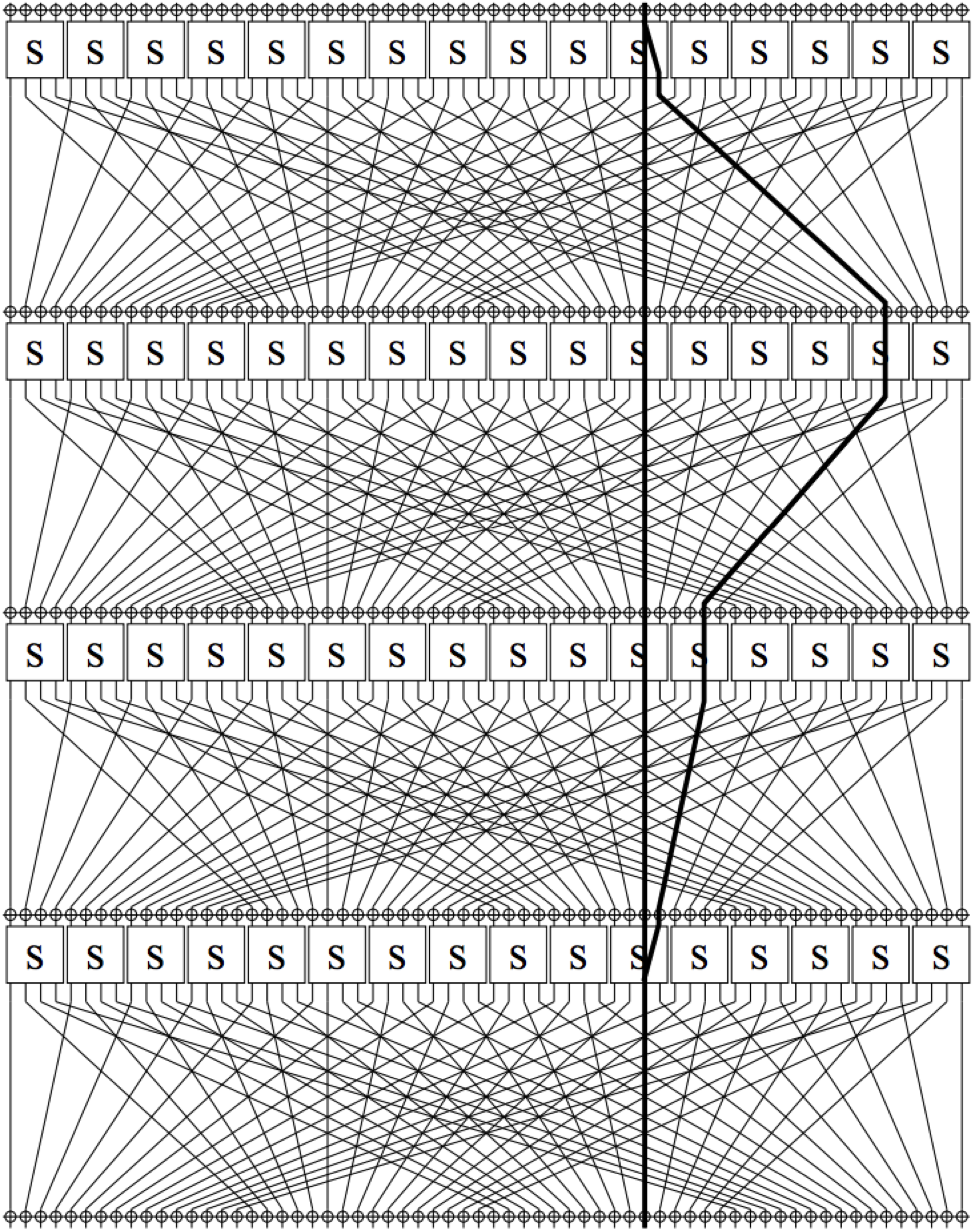
\includegraphics[height=0.62\textheight]{img/PRESENT_Trail.png}
\caption{
Example of an attack on PRESENT that arose due to poor selection of a bitwise permutation. The combination of fixed-points and a low-order permutation results in a trail which minimizes the number of active S-boxes across four rounds \cite{Nakahara2009_PRESENT_Cryptanalysis}.
}
\label{fig:PRESENT_Trail}
\end{figure}


\section{Bitwise Permutations}
\label{appx:BitwisePermutations}
The following bitwise permutations defined by the affine function
\begin{equation*}
\pi(x) = \alpha x + \beta
\end{equation*}
satisfy all required properties listed in Section~\ref{sec:AlgorithmSpec}.
The order of all bitwise permutations listed here is $32$.

\begin{table}[h]
\footnotesize
\begin{tabular}{l|l|l|l|l|l|l|l|l|l|l|l|l|l|l|l|l}
\normalsize $\mathbf{\alpha}$ &   $\mathbf{31}$ &   $\mathbf{33}$ &   $\mathbf{95}$ &   $\mathbf{97}$ &  $\mathbf{159}$ &  $\mathbf{161}$ &  $\mathbf{223}$ &  $\mathbf{225}$ &  $\mathbf{287}$ &  $\mathbf{289}$ &  $\mathbf{351}$ &  $\mathbf{353}$ &  $\mathbf{415}$ & $\mathbf{417}$ &  $\mathbf{479}$ &  $\mathbf{481}$ \\
\hline
\multirow{32}{*}{\begin{sideways}\normalsize \textbf{Corresponding $\beta$ values}\end{sideways}}
&   $15$ &   $16$ &   $15$ &   $16$ &   $15$ &   $16$ &   $15$ &   $16$ &   $15$ &   $16$ &   $15$ &   $16$ &   $15$ &   $16$ &   $15$ &   $16$ \\
&   $31$ &   $48$ &   $31$ &   $48$ &   $31$ &   $48$ &   $31$ &   $48$ &   $31$ &   $48$ &   $31$ &   $48$ &   $31$ &   $48$ &   $31$ &   $48$ \\
&   $47$ &   $80$ &   $47$ &   $80$ &   $47$ &   $80$ &   $47$ &   $80$ &   $47$ &   $80$ &   $47$ &   $80$ &   $47$ &   $80$ &   $47$ &   $80$ \\
&   $63$ &  $112$ &   $63$ &  $112$ &   $63$ &  $112$ &   $63$ &  $112$ &   $63$ &  $112$ &   $63$ &  $112$ &   $63$ &  $112$ &   $63$ &  $112$ \\
&   $79$ &  $144$ &   $79$ &  $144$ &   $79$ &  $144$ &   $79$ &  $144$ &   $79$ &  $144$ &   $79$ &  $144$ &   $79$ &  $144$ &   $79$ &  $144$ \\
&   $95$ &  $176$ &   $95$ &  $176$ &   $95$ &  $176$ &   $95$ &  $176$ &   $95$ &  $176$ &   $95$ &  $176$ &   $95$ &  $176$ &   $95$ &  $176$ \\
&  $111$ &  $208$ &  $111$ &  $208$ &  $111$ &  $208$ &  $111$ &  $208$ &  $111$ &  $208$ &  $111$ &  $208$ &  $111$ &  $208$ &  $111$ &  $208$ \\
&  $127$ &  $240$ &  $127$ &  $240$ &  $127$ &  $240$ &  $127$ &  $240$ &  $127$ &  $240$ &  $127$ &  $240$ &  $127$ &  $240$ &  $127$ &  $240$ \\
&  $143$ &  $272$ &  $143$ &  $272$ &  $143$ &  $272$ &  $143$ &  $272$ &  $143$ &  $272$ &  $143$ &  $272$ &  $143$ &  $272$ &  $143$ &  $272$ \\
&  $159$ &  $304$ &  $159$ &  $304$ &  $159$ &  $304$ &  $159$ &  $304$ &  $159$ &  $304$ &  $159$ &  $304$ &  $159$ &  $304$ &  $159$ &  $304$ \\
&  $175$ &  $336$ &  $175$ &  $336$ &  $175$ &  $336$ &  $175$ &  $336$ &  $175$ &  $336$ &  $175$ &  $336$ &  $175$ &  $336$ &  $175$ &  $336$ \\
&  $191$ &  $368$ &  $191$ &  $368$ &  $191$ &  $368$ &  $191$ &  $368$ &  $191$ &  $368$ &  $191$ &  $368$ &  $191$ &  $368$ &  $191$ &  $368$ \\
&  $207$ &  $400$ &  $207$ &  $400$ &  $207$ &  $400$ &  $207$ &  $400$ &  $207$ &  $400$ &  $207$ &  $400$ &  $207$ &  $400$ &  $207$ &  $400$ \\
&  $223$ &  $432$ &  $223$ &  $432$ &  $223$ &  $432$ &  $223$ &  $432$ &  $223$ &  $432$ &  $223$ &  $432$ &  $223$ &  $432$ &  $223$ &  $432$ \\
&  $239$ &  $464$ &  $239$ &  $464$ &  $239$ &  $464$ &  $239$ &  $464$ &  $239$ &  $464$ &  $239$ &  $464$ &  $239$ &  $464$ &  $239$ &  $464$ \\
&  $255$ &  $496$ &  $255$ &  $496$ &  $255$ &  $496$ &  $255$ &  $496$ &  $255$ &  $496$ &  $255$ &  $496$ &  $255$ &  $496$ &  $255$ &  $496$ \\
&  $271$ &      &  $271$ &      &  $271$ &      &  $271$ &      &  $271$ &      &  $271$ &      &  $271$ &      &  $271$ &      \\
&  $287$ &      &  $287$ &      &  $287$ &      &  $287$ &      &  $287$ &      &  $287$ &      &  $287$ &      &  $287$ &      \\
&  $303$ &      &  $303$ &      &  $303$ &      &  $303$ &      &  $303$ &      &  $303$ &      &  $303$ &      &  $303$ &      \\
&  $319$ &      &  $319$ &      &  $319$ &      &  $319$ &      &  $319$ &      &  $319$ &      &  $319$ &      &  $319$ &      \\
&  $335$ &      &  $335$ &      &  $335$ &      &  $335$ &      &  $335$ &      &  $335$ &      &  $335$ &      &  $335$ &      \\
&  $351$ &      &  $351$ &      &  $351$ &      &  $351$ &      &  $351$ &      &  $351$ &      &  $351$ &      &  $351$ &      \\
&  $367$ &      &  $367$ &      &  $367$ &      &  $367$ &      &  $367$ &      &  $367$ &      &  $367$ &      &  $367$ &      \\
&  $383$ &      &  $383$ &      &  $383$ &      &  $383$ &      &  $383$ &      &  $383$ &      &  $383$ &      &  $383$ &      \\
&  $399$ &      &  $399$ &      &  $399$ &      &  $399$ &      &  $399$ &      &  $399$ &      &  $399$ &      &  $399$ &      \\
&  $415$ &      &  $415$ &      &  $415$ &      &  $415$ &      &  $415$ &      &  $415$ &      &  $415$ &      &  $415$ &      \\
&  $431$ &      &  $431$ &      &  $431$ &      &  $431$ &      &  $431$ &      &  $431$ &      &  $431$ &      &  $431$ &      \\
&  $447$ &      &  $447$ &      &  $447$ &      &  $447$ &      &  $447$ &      &  $447$ &      &  $447$ &      &  $447$ &      \\
&  $463$ &      &  $463$ &      &  $463$ &      &  $463$ &      &  $463$ &      &  $463$ &      &  $463$ &      &  $463$ &      \\
&  $479$ &      &  $479$ &      &  $479$ &      &  $479$ &      &  $479$ &      &  $479$ &      &  $479$ &      &  $479$ &      \\
&  $495$ &      &  $495$ &      &  $495$ &      &  $495$ &      &  $495$ &      &  $495$ &      &  $495$ &      &  $495$ &      \\
&  $511$ &      &  $511$ &      &  $511$ &      &  $511$ &      &  $511$ &      &  $511$ &      &  $511$ &      &  $511$ &      \\
\end{tabular}
\caption{Bitwise permutations satisfying all desired properties}
\label{tab:BitwisePermutations}
\end{table}

\linespread{1}
\selectfont
\chapter{ARX-Based Mixers}
\label{appx:ARX_Mixers}
As part of the design process for the cryptosystem described in this thesis, many ARX-based mixers were analyzed before deciding to switch to a mixer based on matrix multiplication in a Galois field.
None of these ARX-based mixers were able to increase the linear and differential branch numbers from two to three, which is one of our requirements.
For completeness, we enumerate all of the mixers we analyzed here. 

One of the mixers is based on the ARX structure used in Threefish, the block cipher used within SHA-3 candidate Skein \cite{Ferguson2010_SkeinReference}. 
Another is based on the recently released lightweight block cipher Speck that was created by the National Security Agency \cite{Beaulieu2013_Speck}. 
From these ideas, more complex ARX structures were constructed and analyzed.

In all diagrams shown here, the $\mathbf{ROT}$ operation represents all possible nontrivial left and right rotations on a single word. 
Mixers corresponding to every single combination of rotations were analyzed.
The $\boxplus$ symbol denotes addition modulo $2^{16}$.
It is a nonlinear operation due to effect of the carry bit.
The $\oplus$ symbol denotes XOR, as usual.

\begin{figure}[ht]
\centering
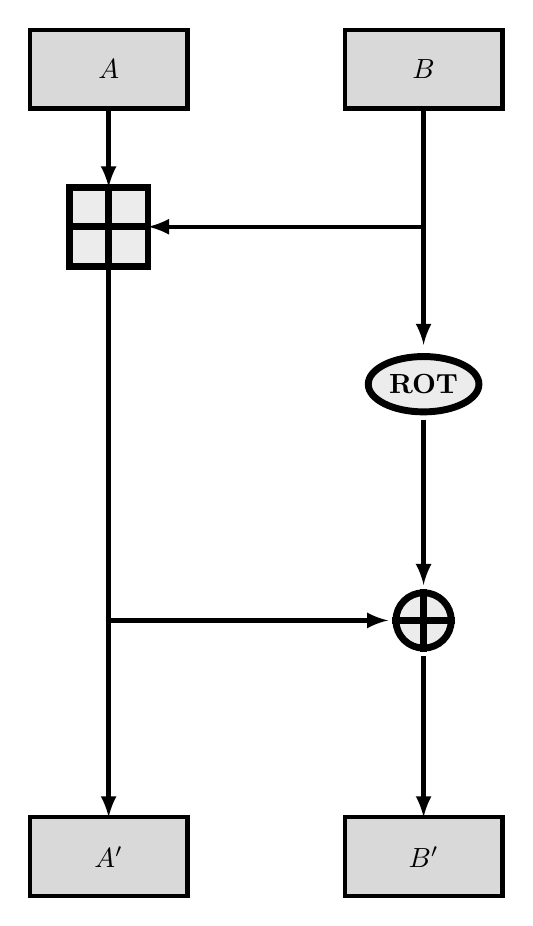
\begin{tikzpicture}[ultra thick,>=latex]
% Reference grid (temporary)
%\draw[help lines] (0,0) grid (16,16);

% Inputs A and B
\drawMixerInputs
\draw[->] (1,15) to (1,14);
\draw[->] (5,15) to (5,12);

% Modular addition
\drawAdder{0.5}{14}

% Right adder input
\draw[->] (5,13.5) to (1.5,13.5);

% Rotation
\drawRot{5}{11.5}

% XOR
\drawXOR{5}{8.5}

% XOR inputs
\draw[->] (1,8.5) to (4.55,8.5);
\draw[->] (5,11.05) to (5,8.95);

% Outputs A' and B'
\draw[->] (1,14) to (1,6);
\draw[->] (5,8.05) to (5,6);
\drawMixerOutputs{10}

\end{tikzpicture}

\caption{Candidate mixer inspired by Threefish}
\end{figure}

\begin{figure}[ht]
\centering
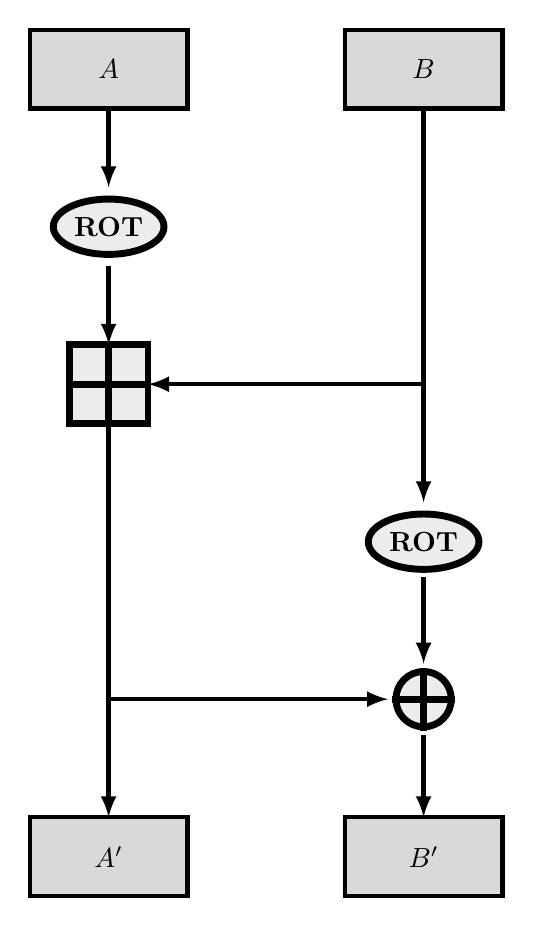
\begin{tikzpicture}[ultra thick,>=latex]
% Reference grid (temporary)
%\draw[help lines] (0,0) grid (16,16);

% Inputs A and B
\drawMixerInputs
\draw[->] (1,15) to (1,14);
\draw[->] (5,15) to (5,10);

% Rotation
\drawRot{1}{13.5}

% Modular addition
\drawAdder{0.5}{12}

% Adder inputs
\draw[->] (1,13) to (1,12);
\draw[->] (5,11.5) to (1.5,11.5);

% Rotation
\drawRot{5}{9.5}

% XOR
\drawXOR{5}{7.5}

% XOR inputs
\draw[->] (1,7.5) to (4.55,7.5);
\draw[->] (5,9.05) to (5,7.95);

% Outputs A' and B'
\draw[->] (1,11) to (1,6);
\draw[->] (5,7.05) to (5,6);
\drawMixerOutputs{10}

\end{tikzpicture}

\caption{Candidate mixer inspired by Speck}
\end{figure}

\begin{figure}[ht]
\centering
\begin{minipage}{.5\textwidth}
\centering
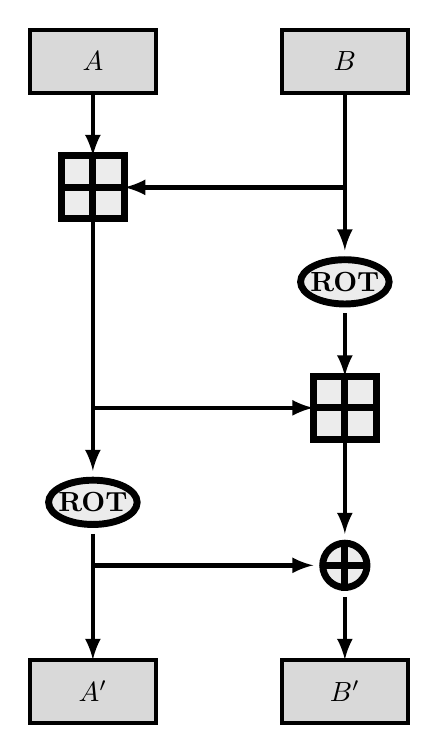
\begin{tikzpicture}[scale=0.8,ultra thick,>=latex]
% Reference grid (temporary)
%\draw[help lines] (0,0) grid (16,16);

% Inputs A and B
\drawMixerInputs
\draw[->] (1,15) to (1,14);
\draw[->] (5,15) to (5,12.5);

% Left adder 
\drawAdder{0.5}{14}
\draw[->] (5,13.5) to (1.5,13.5);

% Rotation
\drawRot{5}{12}

% Right adder
\drawAdder{4.5}{10.5}
\draw[->] (5,11.5) to (5,10.5);
\draw[->] (1,10) to (4.5,10);

% Rotation
\drawRot{1}{8.5}
\draw[->] (1,13) to (1,9);

% XOR
\drawXOR{5}{7.5}
\draw[->] (1,7.5) to (4.5,7.5);
\draw[->] (5,9.5) to (5,8);

% Outputs A' and B'
\draw[->] (1,8) to (1,6);
\draw[->] (5,7) to (5,6);
\drawMixerOutputs{10}
\end{tikzpicture}
\end{minipage}%
%
%
\begin{minipage}{.5\textwidth}
\centering
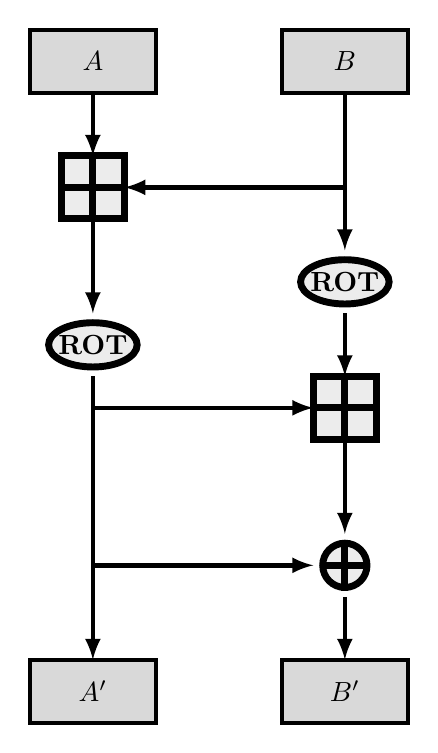
\begin{tikzpicture}[scale=0.8,ultra thick,>=latex]
% Reference grid (temporary)
%\draw[help lines] (0,0) grid (16,16);

% Inputs A and B
\drawMixerInputs
\draw[->] (1,15) to (1,14);
\draw[->] (5,15) to (5,12.5);

% Left adder 
\drawAdder{0.5}{14}
\draw[->] (5,13.5) to (1.5,13.5);

% Rotation
\drawRot{5}{12}

% Rotation
\drawRot{1}{11}
\draw[->] (1,13) to (1,11.5);

% Right adder
\drawAdder{4.5}{10.5}
\draw[->] (5,11.5) to (5,10.5);
\draw[->] (1,10) to (4.5,10);

% XOR
\drawXOR{5}{7.5}
\draw[->] (1,7.5) to (4.5,7.5);
\draw[->] (5,9.5) to (5,8);

% Outputs A' and B'
\draw[->] (1,10.5) to (1,6);
\draw[->] (5,7) to (5,6);
\drawMixerOutputs{10}
\end{tikzpicture}
\end{minipage}
%
%
\begin{minipage}{.5\textwidth}
\vspace{1cm}
\centering
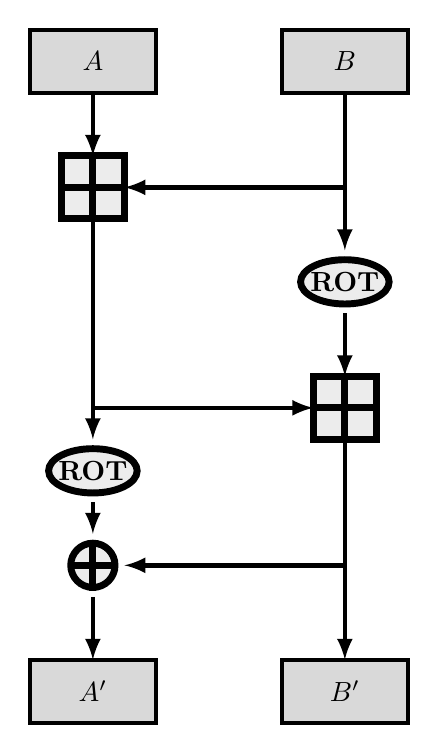
\begin{tikzpicture}[scale=0.8,ultra thick,>=latex]
% Reference grid (temporary)
%\draw[help lines] (0,0) grid (16,16);

% Inputs A and B
\drawMixerInputs
\draw[->] (1,15) to (1,14);
\draw[->] (5,15) to (5,12.5);

% Left adder 
\drawAdder{0.5}{14}
\draw[->] (5,13.5) to (1.5,13.5);

% Rotation
\drawRot{5}{12}

% Rotation
\drawRot{1}{9}
\draw[->] (1,13) to (1,9.5);

% Right adder
\drawAdder{4.5}{10.5}
\draw[->] (5,11.5) to (5,10.5);
\draw[->] (1,10) to (4.5,10);

% XOR
\drawXOR{1}{7.5}
\draw[->] (5,7.5) to (1.5,7.5);
\draw[->] (1,8.5) to (1,8);

% Outputs A' and B'
\draw[->] (1,7) to (1,6);
\draw[->] (5,9.5) to (5,6);
\drawMixerOutputs{10}
\end{tikzpicture}
\end{minipage}%
%
%
\begin{minipage}{.5\textwidth}
\vspace{1cm}
\centering
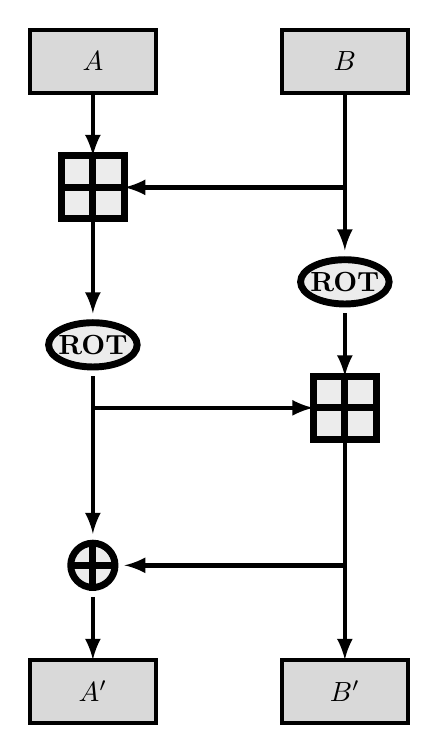
\begin{tikzpicture}[scale=0.8,ultra thick,>=latex]
% Reference grid (temporary)
%\draw[help lines] (0,0) grid (16,16);

% Inputs A and B
\drawMixerInputs
\draw[->] (1,15) to (1,14);
\draw[->] (5,15) to (5,12.5);

% Left adder 
\drawAdder{0.5}{14}
\draw[->] (5,13.5) to (1.5,13.5);

% Rotation
\drawRot{5}{12}

% Rotation
\drawRot{1}{11}
\draw[->] (1,13) to (1,11.5);

% Right adder
\drawAdder{4.5}{10.5}
\draw[->] (5,11.5) to (5,10.5);
\draw[->] (1,10) to (4.5,10);

% XOR
\drawXOR{1}{7.5}
\draw[->] (5,7.5) to (1.5,7.5);
\draw[->] (1,10.5) to (1,8);

% Outputs A' and B'
\draw[->] (1,7) to (1,6);
\draw[->] (5,9.5) to (5,6);
\drawMixerOutputs{10}
\end{tikzpicture}
\end{minipage}
%\caption{Custom candidate mixers with no initial rotation}
\caption{Custom candidate mixers}
\end{figure}

%%%%%%%%%%%%%%%%%%%%%%%%%%%%%%%%%%%%%%%

\begin{comment}
\begin{figure}[p]
\centering
\begin{minipage}{.5\textwidth}
\centering
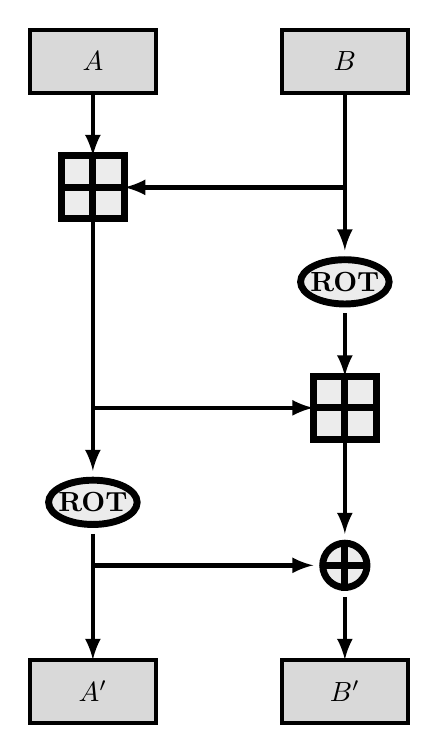
\begin{tikzpicture}[scale=0.8,ultra thick,>=latex]
% Reference grid (temporary)
%\draw[help lines] (0,0) grid (16,16);

% Inputs A and B
\drawMixerInputs
\draw[->] (1,15) to (1,14);
\draw[->] (5,15) to (5,12.5);

% Left adder 
\drawAdder{0.5}{14}
\draw[->] (5,13.5) to (1.5,13.5);

% Rotation
\drawRot{5}{12}

% Right adder
\drawAdder{4.5}{10.5}
\draw[->] (5,11.5) to (5,10.5);
\draw[->] (1,10) to (4.5,10);

% Rotation
\drawRot{1}{8.5}
\draw[->] (1,13) to (1,9);

% XOR
\drawXOR{5}{7.5}
\draw[->] (1,7.5) to (4.5,7.5);
\draw[->] (5,9.5) to (5,8);

% Outputs A' and B'
\draw[->] (1,8) to (1,6);
\draw[->] (5,7) to (5,6);
\drawMixerOutputs{10}
\end{tikzpicture}
\end{minipage}%
%
%
\begin{minipage}{.5\textwidth}
\centering
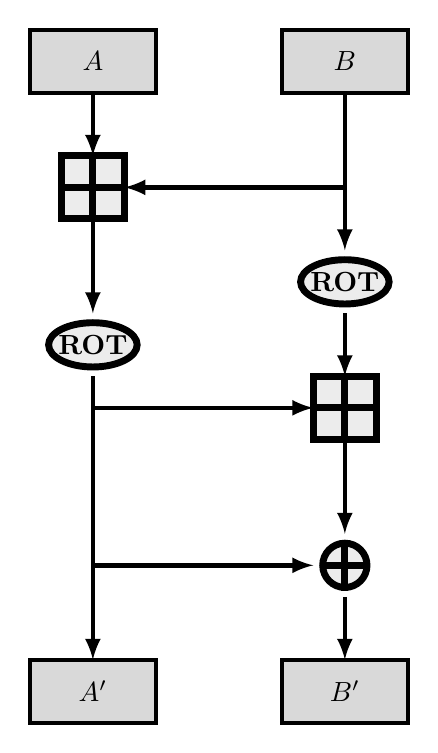
\begin{tikzpicture}[scale=0.8,ultra thick,>=latex]
% Reference grid (temporary)
%\draw[help lines] (0,0) grid (16,16);

% Inputs A and B
\drawMixerInputs
\draw[->] (1,15) to (1,14);
\draw[->] (5,15) to (5,12.5);

% Left adder 
\drawAdder{0.5}{14}
\draw[->] (5,13.5) to (1.5,13.5);

% Rotation
\drawRot{5}{12}

% Rotation
\drawRot{1}{11}
\draw[->] (1,13) to (1,11.5);

% Right adder
\drawAdder{4.5}{10.5}
\draw[->] (5,11.5) to (5,10.5);
\draw[->] (1,10) to (4.5,10);

% XOR
\drawXOR{5}{7.5}
\draw[->] (1,7.5) to (4.5,7.5);
\draw[->] (5,9.5) to (5,8);

% Outputs A' and B'
\draw[->] (1,10.5) to (1,6);
\draw[->] (5,7) to (5,6);
\drawMixerOutputs{10}
\end{tikzpicture}
\end{minipage}
%
%
\begin{minipage}{.5\textwidth}
\vspace{1cm}
\centering
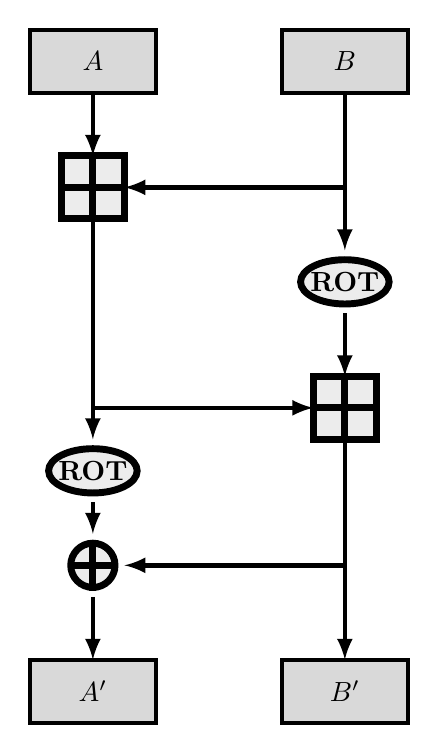
\begin{tikzpicture}[scale=0.8,ultra thick,>=latex]
% Reference grid (temporary)
%\draw[help lines] (0,0) grid (16,16);

% Inputs A and B
\drawMixerInputs
\draw[->] (1,15) to (1,14);
\draw[->] (5,15) to (5,12.5);

% Left adder 
\drawAdder{0.5}{14}
\draw[->] (5,13.5) to (1.5,13.5);

% Rotation
\drawRot{5}{12}

% Rotation
\drawRot{1}{9}
\draw[->] (1,13) to (1,9.5);

% Right adder
\drawAdder{4.5}{10.5}
\draw[->] (5,11.5) to (5,10.5);
\draw[->] (1,10) to (4.5,10);

% XOR
\drawXOR{1}{7.5}
\draw[->] (5,7.5) to (1.5,7.5);
\draw[->] (1,8.5) to (1,8);

% Outputs A' and B'
\draw[->] (1,7) to (1,6);
\draw[->] (5,9.5) to (5,6);
\drawMixerOutputs{10}
\end{tikzpicture}
\end{minipage}%
%
%
\begin{minipage}{.5\textwidth}
\vspace{1cm}
\centering
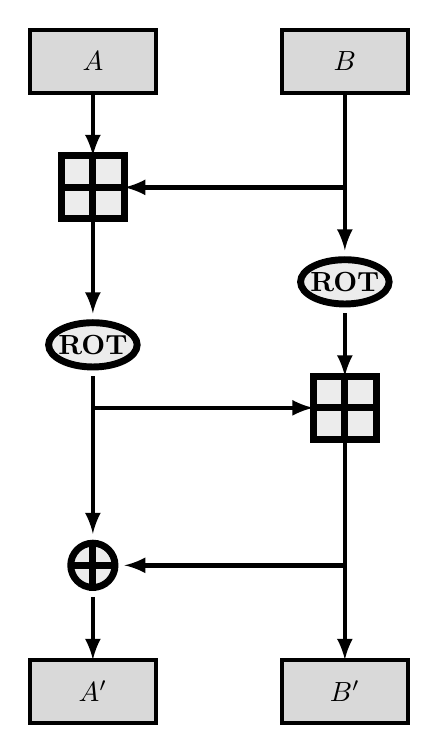
\begin{tikzpicture}[scale=0.8,ultra thick,>=latex]
% Reference grid (temporary)
%\draw[help lines] (0,0) grid (16,16);

% Inputs A and B
\drawMixerInputs
\draw[->] (1,15) to (1,14);
\draw[->] (5,15) to (5,12.5);

% Left adder 
\drawAdder{0.5}{14}
\draw[->] (5,13.5) to (1.5,13.5);

% Rotation
\drawRot{5}{12}

% Rotation
\drawRot{1}{11}
\draw[->] (1,13) to (1,11.5);

% Right adder
\drawAdder{4.5}{10.5}
\draw[->] (5,11.5) to (5,10.5);
\draw[->] (1,10) to (4.5,10);

% XOR
\drawXOR{1}{7.5}
\draw[->] (5,7.5) to (1.5,7.5);
\draw[->] (1,10.5) to (1,8);

% Outputs A' and B'
\draw[->] (1,7) to (1,6);
\draw[->] (5,9.5) to (5,6);
\drawMixerOutputs{10}
\end{tikzpicture}
\end{minipage}
\caption{Custom candiate mixers with initial rotation}
\end{figure}
\end{comment}



\linespread{1}
\selectfont
%------------------------------
% CHAPTER: Known Answer Tests
%------------------------------
\chapter{Known Answer Tests}
\label{appx:KATs}

\makeatletter
\preto{\@verbatim}{\topsep=1em \partopsep=0pt \parskip=0pt \parsep=0pt}
\makeatother

\renewcommand{\arraystretch}{0}

%\begin{table}[ht]
\begin{center}
\input{/p/research/algorithm/KAT_Tables.tex}
\end{center}
%\end{table}

%------------------------------
% APPENDIX: Source Code Listings 
%------------------------------
\chapter{Source Code Listings}
\label{appx:SourceCodeListings}

%------------------------------
% SECTION: AE Algorithm 
%------------------------------
\singlespace
\section{AE Algorithm Software Implementation}

\subsection{State.h}
\lstinputlisting[language=C++]{../../algorithm/State.h}

\subsection{MixerGF.h}
\lstinputlisting[language=C++]{../../algorithm/MixerGF.h}

\subsection{SboxGF.h}
This code was written by Christopher Wood as part of his thesis work in \cite{Wood2013_SboxThesis}; we merely condensed it for brevity here.
\lstinputlisting[language=C++]{../../algorithm/SboxGF.h}

\subsection{Sbox16.h}
This code was written by Christopher Wood as part of his thesis work in \cite{Wood2013_SboxThesis}; we merely condensed it for brevity here.
\lstinputlisting[language=C++]{../../algorithm/SboxGF.h}

\subsection{Permutation.h}
\label{sec:Permutation.h}
\lstinputlisting[language=C++]{../../algorithm/Permutation.h}

\subsection{Sponge.h}
\lstinputlisting[language=C++]{../../algorithm/Sponge.h}

%\subsection{SpongeStream.h}
%\lstinputlisting[language=C++]{../../algorithm/SpongeStream.h}

\subsection{Duplex.h}
\lstinputlisting[language=C++]{../../algorithm/Duplex.h}

\subsection{TestPermutation.cpp}
\lstinputlisting[language=C++]{../../algorithm/TestPermutation.cpp}

\subsection{DuplexKAT.cpp}
\lstinputlisting[language=C++]{../../algorithm/DuplexKAT.cpp}

%------------------------------
% SECTION: Permutation Analyzer 
%------------------------------
\section{Permutation Analyzer}
\lstinputlisting[language=Python]{../../permutations/find_permutations.py}

%------------------------------
% SECTION: P-value Uniformity Test 
%------------------------------
\section{\pval Uniformity Test}
\label{sec:UniformityTestCode}
\lstinputlisting[language=Python]{../../algorithm/uniformity_test.py}



%%%%%%%%%%%%%%%%%%%%%%%%%%%%%%%%%%%%%%%%%%%%%%%%%%%%%%%%%%%%%%%%%%%%%%%%%%%%%%%

\end{document}

